\documentclass[12pt]{article}

%PACKAGES
\usepackage{graphicx}
\usepackage{epstopdf}
\usepackage[english]{babel}
\usepackage[toc,page]{appendix}
\usepackage{listings}
\usepackage{caption}
\usepackage{epsfig}
\usepackage{amsmath} % Required for some math elements 

\usepackage{hyperref}
\usepackage[left=3cm,top=3cm,right=3cm,nohead,nofoot]{geometry}
\usepackage{braket}
\usepackage{datenumber}
\usepackage{placeins}


%COMMANDS

\begin{document}

\begin{center}
\begin{figure}
\centering%
\epsfig{file=general/logo-andes.jpg,scale=0.75}%
\end{figure}
\vspace{3 cm}
\FloatBarrier
\Huge
Laniakea in a Cosmological Context\\
\vspace{3 mm}
or\\
\vspace{3 mm}
Detection of galaxy superclusters in simulated cosmological structures\\  
\vspace{1 cm}
\vspace{3mm}
\Large Sergio Daniel Hern\'{a}ndez Charpak\\

\large
200922618\\
\vspace{1 cm}
\vspace{2mm}
\Large
Advisor: Jaime E. Forero-Romero\\

\normalsize
\vspace{2mm}
\vspace{1 cm}
\today \\
\vspace{1 cm}
\small 
Universidad de los Andes\\
Facultad de Ciencias, Departamento de F\'{i}sica\\
Bogot\'{a}, Colombia\\
\end{center}


\normalsize
\newpage
\section{Acknowledgements}

I would like to thank my advisor, Jaime E. Forero-Romero, for his guidance
 during this process and of course my family,
  Nathalie, Jose Tiberio, Yv\'{a}n David,
  Gabriel Luis, Nico, Dani and all the others for
   their great patience and always good advices. I
    also acknowledge the University of Los Andes
     for its mayor financial support during my
      studies. Finally I couldn't have finish this
       work without the support of Andr\'{e}s,
        Nicol\'{a}s, Jorge and all the special
         friends I am lucky to have. Georges would
          be very happy.


\newpage
\section{Abstract}
Recently Tully et al. (2014)
 \cite{tully_laniakea_2014} used local cosmic flow
 information to define our local supercluster,
  Laniakea. 
In this work we present a study on large
 cosmological N-body
simulations aimed at establishing the significance
 of Laniakea in a
cosmological context.
We explore different algorithms to define
 superclusters from the dark
matter velocity field in the simulation. 
We summarize the properties of the supercluster
 population by their
abundance at a given total mass and its shape
 distributions.
We find that superclusters similar in size and
 structure to Laniakea are
relatively uncommon on a broader cosmological
 context.
We finalize by discussing the possible sources of
 systematics (both in
our methods and in observations) leading to this
 discrepancy.
%TODO make sure it is what it is
\newpage
\tableofcontents
\newpage

\section{Motivation}

We live in the planet Earth. Our planet orbits
 around the Sun in the Solar System, under the
  influence of the gravitational forces. Our Solar
   System forms, along with many other stars and
    systems, our home galaxy, the Milky
    Way. Galaxy themselves, under the
  same forces, form even larger structures. It is
   these structures we call galaxy superclusters. \\
   
   %TODO insert an image to explain the filamentary structure of the univers.

Detecting these galaxy superclusters is a challenging
 task. Observationally there are  There exists
    different algorithms to identify them based on
     physical criteria \cite{gott_iii_map_2005}. One
      possible physical criterion relates the velocity
       flows with the density.
\\

Indeed, due to gravitational attraction, it is possible
 to relate
  velocity fields with density fields. A proposal to
   find galaxy superclusters is to analyze the
    velocity field of galaxies as matter tend to flow to
     dense region. Spacial
      regions where the galaxy flow is convergent
       represent galaxy superclusters.\\
\\
Recently a team of astronomers built a galaxy velocities
 flow map
 of the local universe in a scale of hundreds of million
  light
  years \cite{tully_cosmicflows-2_2013}. In this map, the
   team found converging velocity flows to identify
    identified Laniakea, the galaxy supercluster
     which includes our galaxy, the Milky Way
      \cite{tully_laniakea_2014}. These observations
       are difficult. As a result of these
         difficulties, it is not possible to build a
          statistical sample superclusters obtained
           from the observational approach. 
\\   

\begin{par}
We propose a method to detect galaxy superclusters in
 cosmological simulations following physical criteria
  similar to the one used to define Laniakea. After an
   interpolation of the velocity and density fields we
    apply a region growing algorithm based in predefined
     parameters. We test our method on N-body simulations
      and successfully detect structure we compare to
       Laniakea.\\
We aim to quantify if Laniakea can be
 considered as an atypical structure in
the Universe.   
\\
\end{par}

\begin{par}
The definition of Laniakea by Tully et al
 \cite{tully_laniakea_2014} is based on the
  peculiar velocity flow. Chon et al provide an
   interesting work on a different definition of
    galaxy superclusters, a gravitationally bound
     dense large scale structure
      \cite{chon_characterising_2014} and
       \cite{chon_definition_2015}. On this
        different criteria, Laniakea and how
         Laniakea fits their definition for supercluster
          differs.  \\
\end{par}
\section{Introduction}
\subsection{The Standard Cosmological Model}
\label{cosmo_constants}

\begin{par}

The current standard cosmological model is known the Lambda
 - Cold Matter Model, or $\Lambda$ CDM Model. It assumes Einstein's equations of General Relativity.\cite{bertone_particle_2005}.\\
The
  letter $\Lambda$ makes a reference to the
   cosmological constant $\Omega_{\Lambda}$, which is
    associated with dark energy and the accelerated
     expansion of the Universe according to General
      Relativity. Dark energy is a fairly unknown form of
       energy. It is proposed to explain the accelerated
        rate of expansion of the Universe
         \cite{peebles_cosmological_2003}.
      
The dark matter is a hypothetical type of matter which is
 nor ordinary matter (baryonic matter), nor neutrino
  particles nor dark energy. It is dark as it does not
   seem to produce any radiation (light). There has been
    indirect observations of dark matter as difference
     between gravitational matter implied by velocities
      of stars and observed matter and gravitational
       lensing between others
        \cite{trimble_existence_1987}. Cold means that
         the velocity of the hypothetical fundamental
          particles conforming the dark matter are not
           relativistic. A consequence of this is a
            bottom-up scheme. With bottom-up, we mean
             that small structures merge into one larger
              structure. The opposite would be hot
               matter, meaning that the hypothetical
                fundamental particles could achieve
                 relativistic velocities. In this hot
                  matter model, there is a top-down
                   scheme,
    where an initial large structure breaks into smaller
     structures. \cite{bertone_particle_2005} \\
      
\end{par}

\begin{par}
The simplest $\Lambda$-CDM Model is based on the following 6 general parameters.\\
\begin{enumerate}
\item The Hubble parameter, $H$, defined as the time
 dependent Hubble parameter 
\[
H = \frac{\dot{a}}{a},
\]
where $a(t)$ refers to the scale factor of the Universe. For
 nearby galaxies, H is found to be constant and thus is
  defined as the Hubble constant $H_0$. 
\[
H_0 = 100 \ h \ km \ s^{-1} \ Mpc^{-1} = 67 \pm 7 km \  s^{-1} \ Mpc^{-1} .
\]
$Mpc$ is a cosmological length unit. $1 Mpc = 10^6 \ pc$ where $1 pc = 3.087 \times
  10^{16} m$. $h$ is the dimensionless parameter defined
   by the equation above, $H_0 = 1 \ km \ s^{-1} \ Mpc^{-1} \ h^{-1}$. In this document the length units are $Mpc/h$.

\item Critical density $\rho_{cr}$ found when the cosmological constant is 0 in Einstein's equations, condition needed to have a close universe. $\rho_{cr} = \frac{3H^2}{8 \pi G} = (8.62 \pm 0.12) \times 10^{−27} kg/m^3$. 

\item Baryon density parameter $\Omega_b$. The density of baryonic matter expressed as a fraction of the critical density. $\Omega_b = \frac{\rho_b}{\rho_{cr}} = 0.0486 \pm 0.0010$.

\item Dark matter density parameter $\Omega_c$. The density of dark matter expressed as a fraction of the critical density.$\Omega_c = \frac{\rho_c}{\rho_{cr}} = 0.2589 \pm 0.0057$.

\item Matter density parameter $\Omega_m$ or $\Omega_0$.
 It corresponds to the sum of $\Omega_c$ and
  $\Omega_b$, $\Omega_0 = 0.3089 \pm 0.0062$

\item Dark energy density parameter, cosmological vacuum energy density (or cosmological constant), $\Omega_{\Lambda}$. As we stated before, it is associated to the accelerated rate of expansion of the Universe. $\Omega_{\Lambda} = 0.6911 \pm 0.0062$



\end{enumerate}
The total density parameter, a constraint, is the sum of
 the density parameters and has to be equal to one. $\Omega_{tot} = \Omega_b + \Omega_c + \Omega_{\Lambda} =1$ or $\Omega_{tot} = \Omega_0 + \Omega_{\Lambda} =1$.\\

Another important concept is the redshift. The redshift $z$ can be defined by the following equation\cite{peebles_cosmological_2003}: 
\[
1 + z = \frac{\lambda_{obs}}{\lambda_{em}}.
\] 
It is a measure of the difference between the observed
 wavelength $\lambda_{obs}$ and the wavelength received
  from a distant object $\lambda_{em}$. It is a convenient
   way to label time, with $z=0$ being the
    present time.
\end{par}


\subsection{Cosmic flows and peculiar velocities}
\label{sec:peculiar_vel}
%Describe in detail the Laniakea work and the Methods used
Our method to detect superclusters in cosmological
 simulations is based on the peculiar velocity field
  analysis in a similar fashion as Tully et al. did to find Laniakea \cite{tully_laniakea_2014}
    \cite{tempel_cosmology:_2014}.
\begin{itemize}
\item Basic theoretical considerations
\end{itemize}
\begin{par}
The peculiar velocity is defined as the velocity relative to a rest frame. Its radial component corresponds to the velocity of a galaxy that cannot be explained by the expansion of the Universe. Hubble's law states that nearby galaxies move away from us at a speed proportional to the distance from us (the proportion is Hubble's constant). In other words,
\[ 
v_p = v_{obs} - H_{0} \times d_{obs} .
\]
With $v_p$ the peculiar velocity, $v_{obs}$ and $d_{obs}$ the observed velocity and distance, $H_{0}$ the Hubble constant as described in section \ref{cosmo_constants}.
\end{par}

\begin{par}
From the linear perturbations in the Newtonian limit of
 the $\Lambda$CDM model presented in section
  \ref{cosmo_constants} There is a linear relation
   between the peculiar velocity and the peculiar
    acceleration \cite{padmanabhan_theoretical_2000}.
\[
\vec{v}_p \simeq \frac{2}{3 H \Omega_b} \Omega_{b}^{0.6} \vec{g} .
\]
With $H$ the Hubble parameter,
 $\Omega_b$ the baryonic density parameter and $\vec{g}$ the
  peculiar acceleration with $\vec{g} = \frac{-1}{a}
   \nabla \phi $ with $\phi$ the gravitational
    potential and $a$ the scale factor of the universe.\\
In other words we obtain an expression:
\[ 
\vec{v}_p \propto  - \nabla \phi .
\]
If we take the divergence we obtain:
\[
\nabla \cdot \vec{v}_p \propto - \nabla^2 \phi .
\]
But $\nabla^2 \phi$ responds a Poisson-like equation
 with the density field $\rho$. We can finally write:
\[
\nabla \cdot \vec{v}_p \propto - \rho .
\]
We define the overdensity $\delta$ as the excess density
 in relation with the mean density of the universe.
 $\delta = \rho / \bar{\rho} -1$ with $\bar{\rho}$ the
  mean density. $\delta$ is an adimensional quantity. \\

Our equation for peculiar velocity can be written as
 \cite{tully_laniakea_2014}: 
\[
\nabla \cdot \vec{v}_p = - H_0 f(\Omega_m, \Omega_{\Lambda})\ \delta .
\] 
With $\vec{v}_p$ the peculiar velocity field, $H_0$ the
 Hubble constant, $\Omega_m$ the matter density
  parameter, $\Omega_{\Lambda}$ the Dark matter density
   parameter, $\delta$ the excess density field and $f(\Omega_m, \Omega_{\Lambda})$ a linear function of $\Omega_m$ and $\Omega_{\Lambda}$.\\
   With this relation we can directly link the peculiar
    velocity field and the excess density field. They
     will have related behaviours.
\end{par}


\begin{itemize}
\item Observational methods
\end{itemize}
\begin{par}
We now proceed to describe some of the observational
 methods used Cosmicflows-2
  \cite{tully_cosmicflows-2_2013}. To define Lanieakea,
   the catalogue of
   peculiar velocities is detailed within ~100 Mpc with
    data covering out to ~400 Mpc. Six main methods
     were jointly used to estimate the galaxy
      distances.	\\
 \begin{enumerate}
 \item Cepheid Period-Luminosity
      Relation (Cepheid PLR) applied to the Hubble
       Space Telescope (HST) distance scale key
        project. The HST data is covers distances
         within 10 Mpc. Their observation can be
          difficult due to luminosities of neighbouring
           objects.\\
              
  \item Tip of Red Giant Branch (TRGB). Red Giants are
   stars 
     fainter than the Cepheids but are located in
      regions with small luminosity noise. This method,
       complementary to the Cepheid PRL method covers
        distances within 10 Mpc.\\
        
  \item Surface Brightness Fluctuation (SBF) method measures the variance in the distribution of light
    emitted in a galaxy. The noisy fluctuations we
     observe are proportional to the distance of the
      galaxy. This method covers distances within 100
       Mpc.\\
  
  \item Elliptical fundamental plane. The quality of these measurements is not very
  good. Despite of that, it can be used for large
   samples of galaxies in a large volume.\\
   
   \item Spiral luminosity-rotation. This method also provides less accurate
  distances, but can be applied to large sets of
   galaxies.\\
   
  \item Supernovae Ia method.
These supernovas are very bright and can been seen from
 great distances. The quality of these measurements is
  good and can cover large distances. Nevertheless,
   samples of these supernovas
   are small.
\end{enumerate}     

\end{par}


\begin{par}
Finally, after the observation were made, a Wiener Filter was applied. A Wiener filtering method is a tool to reconstruct
 large scale structure information from some of the incomplete
  and noisy data \cite{zaroubi_wiener_1995}. It  was
   applied by Tully et al. \cite{tully_laniakea_2014}
    to  to obtained a better Signal/Noise proportion in
     the peculiar velocity field from the Cosmicflows-2 observations.\\
\end{par}


\subsection{The V-Web Algorithm}
\label{sec:v_web}
The contour of the region of Laniakea were reconstructed
 using the V-web Algorithm \cite{tully_laniakea_2014}.
  The basis of our method for the
  detection superclusters in cosmological simulation is
   the V-Web Algorithm, first introduced by Hoffman et al \cite{hoffman_kinematic_2012}.\\

%Reference 
This algorithm is deeply
  connected to the velocities. Its core is the
   shear velocity tensor  defined as:\\
$$
\Sigma _{\alpha\beta} = -\frac{1}{2 H_0} \left( \frac{\partial v_{\alpha}}{\partial x_{\beta}} + \frac{\partial v_{\beta}}{\partial x_{\alpha}} \right) ,
$$
With $v_{\alpha}$ and $x_{\alpha}$ representing the $\alpha$ component the comoving peculiar velocity and the comoving position, respectively.  \\

$\Sigma _{\alpha\beta}$ can be represented by a $3 \times
 3$ symmetric matrix with real values. This makes it
  possible to diagonalize it and find its 3 eigenvalues.\\
These eigenvalues $\lambda_1$, $\lambda_2$ and
 $\lambda_3$ carry information about the motion of the
 fluid. By convention they are ordered such as
  $\lambda_1 > \lambda_2 >\lambda_3$. The V-Web scheme
   refers to the web classification based on how many of
    these eigenvalues are above a predefined threshold.
     Respectively if 0, 1, 2 or 3 eigenvalues are above
      the threshold the point is classified as a void,
       sheet, filament or knot. \\
       
Our method uses indirectly these eigenvalues through the
 Fractional Anisotropy and the trace of 
 $\Sigma _{\alpha\beta}$.


\subsection{Fractional Anisotropy (FA) and Velocity Divergence (VDH)}
\label{sec:FA_trace}

Our method uses on the Fractional Anisotropy (FA) and the trace of the Velocity Shear Tensor.\\


The Fractional Anisotropy (FA) was first conceived in the
 medical context by Peter Basser
  \cite{basser_inferring_1995}. Libeskind et al
   \cite{libeskind_velocity_2013} first introduced the FA
    in the cosmological context. It has been used as
    a tracer of cosmic voids by Bustamante et al.
     \cite{bustamante_tensor_2015}.\\
    
The FA can be written as:
\[
FA = \frac{1}{\sqrt{3}} \sqrt{\frac{( \left( \lambda_1 - \lambda_3 \right)^2 + \left( \lambda_2 - \lambda_3 \right)^2 + \left( \lambda_1 - \lambda_2 \right)^2  )}{\lambda^{2}_1 + \lambda^{2}_2 + \lambda^{2}_3}} ,
\]
With $\lambda_1$, $\lambda_2$ and $\lambda_3$ the
 eigenvalues obtained from the V-Web algorithm. The FA is
  dimensionless and takes values between 0 and
   1. We
  interpret FA = 0 as an isotropic velocity distribution (where $\lambda_1 = \lambda_2 =
    \lambda_3$) and FA = 1 as a highly anisotropic
     velocity distribution. 

\begin{itemize}
\item The trace of the Velocity Shear Tensor (VDH)
\end{itemize}

We describe in section \ref{sec:peculiar_vel} the divergence of the peculiar velocity field is proportional to the overdensity:
\[
\nabla \cdot \vec{v}_p \propto - \delta
\]

The trace of the velocity shear tensor $\Sigma
 _{\alpha\beta}$, $\lambda_1 + \lambda_2 + \lambda_3$ is
 equal to the divergence of the velocity divided by a
  factor $H_0$, the Hubble constant.
\[
\lambda_1 + \lambda_2 + \lambda_3 = \frac{- \nabla \cdot \vec{v}}{H_0} .
\]
This is an dimensionless quantity, proportional to the overdensity $\delta$.\\

We name the trace of $\Sigma_{\alpha\beta}$ or $\frac{- \nabla \cdot \vec{v}}{H_0}$ as VDH which states as
 Velocity Divergence divided by the Hubble constant. 

In the next section we observe how we use the FA and VDH
 to find superclusters in cosmological simulations.

\section{Methods}

\begin{par}
We run our own cosmological N-body simulations. We
 proceed to compute the FA and VDH from the simulations
  data in a series of intermediate steps. Finally, our
   algorithm uses the FA and VDH computed from N-body
    simulations to detect superclusters.
\end{par}

\begin{par}
Our code and algorithm are available for the
  public in Github
   \url{https://github.com/sercharpak/Monografia/}
\end{par}


\subsection{Cosmological Simulations}\label{sec:sims}
\begin{par}
To make our own cosmological simulations we use the N-Body simulation software Gadget-2
 \cite{springel_gadget_2_2005}
widely used in the scientific community to
 generate different cubic boxes of dark matter
  particles
  (DM). \\

By DM particle we mean a computational particle which only interacts through gravity
interaction. In the simulation each particle
 represents a fluid element. The DM particles are
placed in a 3D grid layout first and then are
 perturbed following a Gaussian distribution
before the simulation start, during the initial
 conditions generation. Once the simulation starts, the particles interact only with gravity. Gadget-2 simulates this fluid. The simulations ran on the HPC cluster at
   UNIANDES.
  The main properties (boxsize, number of
   particles, number of CPUs used and time of the
    simulation) are described in table
     \ref{tab:sims}. \\
\end{par}

\begin{par}
We are looking for structures of the same order of
 magnitude of Laniakea (radius of 80 Mpc/h). Our simulations need to be
   of at least the same order of magnitude. We also
    need a sufficient number of DM particles to
     be able to describe the density field on the smaller scales probed by observations (around 5 Mpc/h). From these constraints we decided to run three simulations as listed in table \ref{tab:sims}. 
\end{par}
\begin{table}[ht]
    \centering
    \begin{tabular}{|c|c|c|c|c|}
        Name & Boxsize [Mpc/h] & DM particles & \# CPU & Time [hours] \\
        Medium & 500 & $512^{3}$ & 48 & ~ 10 \\
        Small (Dense) & 250 & $512^{3}$ & 48 & ~ 6  \\
        Medium (Dense) & 500 & $1024^{3}$ & 48 & ~ 80\\
    \end{tabular}
    \caption{Different N-body Simulations}
    \label{tab:sims}
\end{table}
\FloatBarrier


The initial conditions were generated using Volker
 Springel's N-Genic software. For the initial
  conditions we specify the cosmological constants
   described in section \ref{cosmo_constants}. They
    are described in table \ref{tab:consts}\\.
   
  
 \begin{table}[ht]
    \centering
    \begin{tabular}{|c|c|c|c|}
        $\Omega_0$ & $\Omega_{\Lambda}$ & $\Omega_b$ & H \\
        0.3 &  0.7 & 0 & 0.7 \\
    \end{tabular}
    \caption{Cosmological Constants in the N-body Simulations}
    \label{tab:consts}
\end{table}
\FloatBarrier

As we specify in section \ref{cosmo_constants}, $\Omega_0$  corresponds to the Cosmological matter
 density parameter in units of the critical density at
red shift z = 0. $\Omega_{\Lambda}$ is the cosmological
 vacuum energy density (cosmological constant) in
  units of the critical density at red shift z = 0 (present). 
%Relevant only for comoving integration. 
For the standard cosmological model, $\Omega_0$ + $\Omega_{\Lambda}$ = 1.
 $\Omega_b$ is the baryon density in units
  of the critical density at red shift z = 0. Finally, H denotes the Hubble
    constant at red shift z=0 in  units of 100 
    $km$ $s^{-1}$
     $Mpc^{-1}$. 

We then use different algorithms to identify the
 superclusters within the simulation.\\

\subsection{Intermediate Steps} \label{sec:approaches}
%Opening the section



\begin{par}
\footnote{
We also explored an approach of
 the magnitude of the velocity in the different
  simulations. We work with all the particles and
   points given by the simulation. As our final
    results are not based in this naive approach
     we leave it as an appendix here. It is
      explained in further detail in Appendix
       \ref{App:App_Speed}}.
Our algorithm uses the FA and VDH computed from the N-
body simulations. There are three steps involved before.
 First, the interpolation of the particle data
  informations into a grid. Second, the V-web computation
   on this grid. Finally, the computation of the FA and
    VDH on this grid. 
\end{par}


\begin{itemize}
\item The Cloud In Cell (CIC) interpolation method
\end{itemize}
\begin{par}
The Cloud In Cell (CIC) is a method to interpolate a
 quantity such as the density in a grid. The (CIC) method
 is a derivation of the
 Particle in Cell (PIC) method, a Particle Mesh (PM)
  method, first introduced by Francis Harlow in the
   1950's in the field of computational fluid dynamics
    \cite{harlow1964particle}. CIC is very popular
     among the scientific community
      \cite{grigoryev_numerical_2002}. We form, in our
       case, a $N^3$ grid. This grid is superpose with
        the cubic
      box resulting from the simulation. We then form
       particle clouds (cubes in our case) around each
        particle. For each particle cloud, each cell
         where the particle cloud superposes is
          assigned a weighted part of the physical
           quantity we look to mesh proportional to the
            superposed volume (in 2-D, superposed
             area). A function can then be applied to
              smooth the obtained field. We perform
               this CIC
            for the density field and the velocity
             field. In figure \ref{fg:cic_explain} a
              graphical explanation is provided for the
               2-D case.  \\
\end{par}

\begin{figure}[ht]
\begin{center}
\includegraphics[width=0.6\textwidth]{general/CIC_Explain_bigger} % Include the image placeholder.png
\caption{Visualization of the Cloud In Cell Method (CIC)}
\label{fg:cic_explain}
\end{center}
\end{figure}
\FloatBarrier

\begin{itemize}
\item The V-Web scheme, the FA and the VDH
\end{itemize}
\begin{par}
We describe the V-Web scheme in section \ref{sec:v_web}
 and the FA and VDH in section \ref{sec:FA_trace}.
The FA gives us a dimensionless quantity to analyse
 isotropy and the VDH gives us a also another
  dimensionless quantity which behaves in a similar
   fashion as the matter overdensity $\delta$.
\end{par}


\begin{par}
In summary, our approach follows the steps:
\end{par}

\begin{enumerate}
\item Calculate the density field using CIC on the simulation data.
\item Calculate the velocity field using CIC on the simulation data.
\item Use finite differences to compute the velocity shear tensor $\sum_{\alpha \beta}$.
\item Diagonalize $\sum_{\alpha \beta}$ and find its eigenvalues $\lambda_i$ and eigenvectors $\hat{u}_i$
\item Compute the FA and VDH grids as described in section \ref{sec:FA_trace} 
\item Apply the algorithms described in section \ref{sec:algorithms} to find the superclusters
\item Extract the properties (volume, shape, mass) from the superclusters
\item Compare the superclusters detected in the simulation to Laniakea
\end{enumerate}


%Closing the section
\begin{par}
This methodology is very close with the approach
 used to define Laniakea
  \cite{tully_laniakea_2014} which is important to
   validate our later comparison of Laniakea with
    our detected structures.
\end{par}

\subsection{Superclusters Finding Algorithms}\label{sec:algorithms}

Our main algorithm is a region growing algorithm
 as described by Gonzalez
  \cite{gonzalez_digital_2008} mainly used in
   image segmentation.
\subsubsection{Region Growing Algorithm: Basic Description}

\begin{par}
The region growing algorithm is used to identify regions sharing common properties. First we identify points, as few as possible, which we know for sure are contained in these regions. These points are the seeds of our regions. We then define a certain growth predicate, if the neighbours of a seed validate this predicate they are considered as members of the group. These new members are then treated as seeds and ask their own neighbours if they validate the predicate. This goes on until all the points have been evaluated or until a limit defined by the user is reached.
\end{par}

\begin{par}
We can write in a more formal way:
\end{par}

\begin{par}
$f(x,y,z)$ denotes the input data. $S(x,y,z)$ denotes a seed array, with
value 1 where the particle can be define as a seed and 0 where not. $S(x,y,z)$ is the
same size of $f(x,y,z)$. $Q$ denotes a predicate which is to be apply to the
input data and determines if the region which
 starts at the seeds grows or
not. 
\end{par}

\begin{enumerate}
	\item We search for seeds from $f(x,y,z)$ based in a criterion
	\item For each detected seed, we change the values of $S(x,y,z)$ to 1 at the seed's coordinates.
	\item For each detected seed, we iterate its neighbors if they validate the predicate $Q$.
    \item If the particle $c$ at $x_c, y_c, z_c$ satisfies $Q$, it is marked as part of the region, $S(x_c, y_c, z_c) = 1$
    \item Apply the algorithm to $c$, and so on
     (Recursion).
\end{enumerate}

\begin{par}
The algorithm is based on a connectivity concept (definition of
neighbours). Here we are working on a 4-connectivity. 4
connectivity means that no diagonal particles are considered as
neighbours. The following matrix shows this principle in a 2
dimensional case. Only the elements labelled as 1 are considered as
neighbours of the center $C$.
\end{par}

\[ 
\begin{bmatrix} 
    0 & 1 & 0 \\
    1 & C & 1 \\
    0 & 1 & 0\\
\end{bmatrix} 
\]

\begin{par}
So, if a particle is in coordinates $(x,y,z)$ its neighbours are
$(x-1,y,z)$, $(x+1,y,z)$, $(x,y-1,z)$, $(x,y+1,z)$, $(x,y,z-1)$
and $(x,y,z+1)$.
\end{par}

\begin{par}
Another widely used connectivity is the 8-connectivity. As it is
intuitive, in 8-connectivity, the diagonal particles are also
considered as neighbours. We decided to use 4-connectivity to
simplify our own implementation.
\end{par}




\subsubsection{Region Growing Algorithm with the FA and the trace of the velocity shear tensor}\label{sec:own_impl_descr}
Our implementation is based in the FA and the VDH. It is uses 4-connectivity as described before.

\begin{itemize}
    \item Seeds
\begin{par}
We are looking for overdense structures. Therefore we will look
for particles with $VDH \geq 1.0$.  We also want to analyse how
the FA fits. We know that the centres of our structures should be
fairly isotropic so we will explore seeds with FA lesser than a
threshold. We will perform several runs of the algorithm, so we
can explore the different criterion for the choice of the seeds.
These can be seen in table \ref{tab:seeds_FA_Trace}. 
\end{par}
 \begin{table}[ht]
    \centering
    \begin{tabular}{|c|c|c|c|}
        $FA_{seed}$ & $VDH_{seed}$ \\
        0.5 &  1.0 \\
        0.6 &  1.0 \\
        0.7 &  1.0 \\
        0.8 &  1.0 \\
        0.9 &  1.0 \\
    \end{tabular}
    \caption{Different values of the FA and VDH for the choice of the seeds}
    \label{tab:seeds_FA_Trace}
\end{table}
\FloatBarrier

\item Labelling the regions
\begin{par}
We label groups as a function of its respective
 seed to extract properties (volume, shape, mass)
  for each one of them.
\end{par}

\item Predicate $Q$

\begin{par}
We define, as we did for the
choice of the seeds, thresholds for the FA and for VDH. If
the neighbour cell validates these thresholds, and hasn't been
labelled yet, it is labelled as the group of the seed particle. So
in other words: \\

\begin{center}
$Q: \left( FA (x,y,z) \leq Thresh_{FA} \right)$ AND
$\left( VDH (x,y,z) \geq Thresh_{VDH} \right)$ 
\end{center}
As we are looking for overdense regions (no voids) we define the
threshold for VDH as 0.0. As we are exploring the different
values for the FA. each run will follow a row of the table \ref{tab:search_FA_Trace}.
\end{par}

\begin{table}[ht]
    \centering
    \begin{tabular}{|c|c|c|c|}
        $FA_{growth}$ & $VDH_{growth}$ \\
        0.5 &  0.0 \\
        0.6 &  0.0 \\
        0.7 &  0.0 \\
        0.8 &  0.0 \\
        0.9 &  0.0 \\
    \end{tabular}
    \caption{Different values of the FA and VDH for the growth of the regions}
    \label{tab:search_FA_Trace}
\end{table}
\FloatBarrier

\end{itemize}



%\subsubsection{FoF with the FA and Overdensity}\label{sec:fof_impl_descr}
\begin{par}
\footnote{
A simplified version code can be seen in appendix \ref{App:own_impl_code}. Results of this
  implementation can be seen in appendix
   \ref{sec:results_own_impl}.
}
Finally to find the groups we used the Friends-of-Friends (FoF) algorithm.
\end{par}

\begin{par}
The FoF algorithm looks at the distances between points in a given
set. If the distance between a point $a$ and a point $b$ is less
than a predefined threshold, $a$ and $b$ now form a region. For a
region to be created by the FoF algorithm it also needs to have a
predefined minimum number of members. 
\end{par}

\begin{par}
We choose as set of points all the
particles which validate the predicate $Q$ (following table
\ref{tab:search_FA_Trace}, as maximum distance the distance
between one particle and its neighbours as described by
4-connectivity. And we use the FoF algorithm to form the groups. 
\end{par}
\begin{par}
We search for the seeds following table \ref{tab:seeds_FA_Trace}
and obtain a list of the seeds. We then proceed to validate which
of the groups obtained by the FoF is a valid group. To be
considered as a valid group, it needs to contain at least one seed
particle. This procedure allow us to take care of the case where
two seeds form two groups which eventually get together. Now we
can make sure these groups are merged into one and there is no
need to search for this case individually.
\end{par}


\section{Results}

The following results correspond to our
 \textbf{Small (Dense)} described in table
  \ref{tab:sims}.
  
\subsection{Fractional Anisotropy and Divergence in the Simulation}

\subsubsection{Fractional Anisotropy}
 We compute the FA after interpolating the density and velocity fields on a $256^{3}$
   grid using the CIC method and applying the V-Web algorithm. Figure \ref{fg:hist_FA} shows the FA histogram. Figure
      \ref{fg:cut_FA} shows a 2-D cut of the FA grid.
%Histogram and cut
\begin{figure}[ht]
\centering
\begin{minipage}{.5\textwidth}
  \centering
  \includegraphics[width=0.8\textwidth]{simulation/FA_hist_sim.png}
  \caption{FA Histogram in the simulation}
\label{fg:hist_FA}
\end{minipage}%
\begin{minipage}{.5\textwidth}
  \centering
  \includegraphics[width=0.95\textwidth]{simulation/FA_cut_i_10.png}
  \caption{A cut of the FA in the x axis}
\label{fg:cut_FA}
\end{minipage}
\end{figure}
\FloatBarrier

\begin{par}
As we saw in section \ref{sec:FA_trace}, we
 expect to have few highly isotropic particles.
  The histogram in figure \ref{fg:hist_FA} we confirms this expectation.\\
The 2-D cut of the FA in figure \ref{fg:cut_FA} shows the filamentary structures we would
  expect of the Cosmic Web. This cut is very
   similar to the ones presented by  Bustamante et
   al.  \cite{bustamante_tensor_2015} in their
    work. This is a good indicator that our
     simulation, CIC procedure V-Web application
      and FA forming are correctly executed.
       Bustamante et. al  explain that void
        regions should have a $FA < 0.95$. We expect
         superclusters to have a similar isotropic
          behaviour as voids. Therefore we explore
          similar FA values in our method. To make sure
           we do not find voids we make use of the VDH.
\end{par}


\subsubsection{VDH, Velocity Divergence}
As we did for the FA, we visualize the
 histogram (Figure \ref{fg:hist_Trace}) and a
  2-D cut (Figure \ref{fg:cut_Trace}) of the VDH.

%Histogram and cut
\begin{figure}[ht]
\centering
\begin{minipage}{.5\textwidth}
  \centering
  \includegraphics[width=0.8\textwidth]{simulation/Trace_hist_sim.png} % Include the image placeholder.png
\caption{VDH Histogram in the simulation}
\label{fg:hist_Trace}
\end{minipage}%
\begin{minipage}{.5\textwidth}
  \centering
  \includegraphics[width=0.95\textwidth]{simulation/Trace_cut_i_10.png}
  \caption{A cut of the VDH in the x axis}
\label{fg:cut_Trace}
\end{minipage}
\end{figure}
\FloatBarrier


\begin{par}
The VDH distribution is symmetric
 around 0.0. As we are searching for overdense
  structures (superclusters) we can then diminish
   our search space to half of it only by
    selecting the points with $VDH > 0.0$. \\
Observing a 2D cut of the Velocity Divergence as shown in
 figure \ref{fg:cut_Trace} also gives a good idea
  of good idea of the Cosmic Web as we can easily
   recognize filaments (highly underdense, $VDH
    \leq - 1.0$) and highly overdense regions
     ($VDH \geq 1.0$). Our candidates
      for seeds of supercluster structures are the highly
       overdense regions with $VDH \geq 1.0$.
\end{par}


\subsection{Region Growing Algorithm and FoF with the FA and VDH}
%The real results I got
\begin{par}
We apply all the combinations
   for thresholds in table \ref{tab:seeds_FA_Trace}
    (seeds)  and table \ref{tab:search_FA_Trace}
     (growth). \\
\end{par}

\begin{par}
Our algorithms run successfully on a regular
 laptop. Two examples of detected superclusters are
  shown individually on figure
   \ref{fg:detected_small_51_90} and at the scale
    of the simulation (of size 250 Mpc/h) on figure
     \ref{fg:detected_scale_51_90}. Finally we can
      see all the detected regions on the
       simulation with one selection of thresholds
        in figure \ref{fg:detected_all_51_90}.
\end{par}

\begin{figure}[ht]
\centering
\begin{minipage}{.5\textwidth}
  \centering
  \includegraphics[width=0.9\textwidth]{groups/3d/seeds_FA_5/region_2184_small_seeds_FA_05_Trace_10_search_FA_09_Trace_00_.png} % Include the image placeholder.png
\end{minipage}%
\begin{minipage}{.5\textwidth}
  \centering
  \includegraphics[width=0.9\textwidth]{groups/3d/seeds_FA_5/region_4094_small_seeds_FA_05_Trace_10_search_FA_09_Trace_00_.png}
\end{minipage}
\caption{Two detected superclusters in the Small (Dense) simulation with thresholds: Seed (FA: 0.5, Div: 1.0) and Growth (FA: 9.0, Div:0.0). }
\label{fg:detected_small_51_90}
\end{figure}
\FloatBarrier

\begin{figure}[ht]
\centering
\begin{minipage}{.5\textwidth}
  \centering
  \includegraphics[width=0.9\textwidth]{groups/3d/seeds_FA_5/region_2184_scale_seeds_FA_05_Trace_10_search_FA_09_Trace_00_.png} % Include the image placeholder.png
\end{minipage}%
\begin{minipage}{.5\textwidth}
  \centering
  \includegraphics[width=0.9\textwidth]{groups/3d/seeds_FA_5/region_4094_scale_seeds_FA_05_Trace_10_search_FA_09_Trace_00_.png}
\end{minipage}
\caption{Two detected superclusters in the Small (Dense) simulation at scale with thresholds: Seed (FA: 0.5, Div: 1.0) and Growth (FA: 9.0, Div:0.0). }
\label{fg:detected_scale_51_90}
\end{figure}
\FloatBarrier

\begin{figure}[ht]
\begin{center}
  \includegraphics[width=0.9\textwidth]{groups/3d/seeds_FA_5/regions_nonoise_seeds_FA_05_Trace_10_search_FA_09_Trace_00_.png}
\caption{All the superclusters detected in the Small (Dense) simulation with thresholds: Seed (FA: 0.5, Div: 1.0) and Growth (FA: 9.0, Div:0.0). Different colors indicate different regions.}
\label{fg:detected_all_51_90}
\end{center}
\end{figure}
\FloatBarrier

\begin{par}
We can observe from figures
 \ref{fg:detected_all_51_90},
  \ref{fg:detected_scale_51_90} and
   \ref{fg:detected_small_51_90} that the
    structures have different shapes and sizes.
     There are no hints for a specific shape and
      size. In the next section we analyse with more detail how
       FA thresholds influence these results.
\end{par}

\subsubsection{Influence of the FA in the seeds}
\label{sec:infl_FA_seed}
\begin{par}
We proceed to observe how changing the FA threshold
 for the seed selection process described in
  section \ref{sec:algorithms} influences the
   detected structures. 
\end{par}

\begin{figure}[ht]
\centering
\begin{minipage}{.45\textwidth}
  \centering
  \includegraphics[width=0.9\textwidth]{groups/3d/seeds_FA_5/regions_nonoise_seeds_FA_05_Trace_10_search_FA_09_Trace_00_.png}
\end{minipage}%
\begin{minipage}{.45\textwidth}
  \centering
  \includegraphics[width=0.9\textwidth]{groups/3d/seeds_FA_6/regions_nonoise_seeds_FA_06_Trace_10_search_FA_09_Trace_00_.png}
\end{minipage}
\begin{minipage}{.45\textwidth}
  \centering
  \includegraphics[width=0.9\textwidth]{groups/3d/seeds_FA_7/regions_nonoise_seeds_FA_07_Trace_10_search_FA_09_Trace_00_.png}
\end{minipage}
\begin{minipage}{.45\textwidth}
  \centering
  \includegraphics[width=0.9\textwidth]{groups/3d/seeds_FA_8/regions_nonoise_seeds_FA_08_Trace_10_search_FA_09_Trace_00_.png}
\end{minipage}
\caption{Effect of increasing the FA threshold in the seed selection. From upper left to down right the FA for the seeds are: 0.5, 0.6, 0.7 and 0.8. The growth FA is 0.9 and $tr \left(\sum_{\alpha\beta}\right)$ is 0.0. The $tr \left(\sum_{\alpha\beta}\right)$ for the seeds is 1.0.} \label{fg:3D_FA_seeds}
\end{figure}
\FloatBarrier

\begin{par}
In figure \ref{fg:3D_FA_seeds}, we observe qualitatively
 increasing the FA threshold in the seed selection
  increases strongly the number of regions detected. This
   indicates that the number of seeds for the algorithm
    increases as well with the FA threshold in the seed
    selection. The FA histogram (figure \ref{fg:hist_FA})
     shows this as well as most part of the particles
      have a high value of FA.
\end{par}


\subsubsection{Influence of the FA in the growth}
\label{sec:infl_FA_growth}
\begin{par}
We now observe how changing the FA threshold
 for the growth space affects our results. 
\end{par}

\begin{figure}[ht]
\centering
\begin{minipage}{.45\textwidth}
  \centering
  \includegraphics[width=0.9\textwidth]{groups/3d/seeds_FA_6/regions_nonoise_seeds_FA_06_Trace_10_search_FA_06_Trace_00_.png}
\end{minipage}%
\begin{minipage}{.45\textwidth}
  \centering
  \includegraphics[width=0.9\textwidth]{groups/3d/seeds_FA_6/regions_nonoise_seeds_FA_06_Trace_10_search_FA_07_Trace_00_.png}
\end{minipage}
\begin{minipage}{.45\textwidth}
  \centering
  \includegraphics[width=0.9\textwidth]{groups/3d/seeds_FA_6/regions_nonoise_seeds_FA_06_Trace_10_search_FA_08_Trace_00_.png}
\end{minipage}
\begin{minipage}{.45\textwidth}
  \centering
  \includegraphics[width=0.9\textwidth]{groups/3d/seeds_FA_6/regions_nonoise_seeds_FA_06_Trace_10_search_FA_09_Trace_00_.png}
\end{minipage}
\caption{Efect of increasing the FA threshold in the growth. From upper left to down right the FA for the growth is: 0.6, 0.7, 0.8 and 0.9. The seed FA is 0.6 and VDH is 1.0. The VDH for the growth is 0.0.} \label{fg:3D_FA_growth}
\end{figure}
\FloatBarrier

\begin{par}
 Figure \ref{fg:3D_FA_growth} shows qualitatively how augmenting the FA thresholds for the growth changes drastically the volumes of the regions detected, specially from the transition form FA threshold 0.8 to 0.9. This can also be seen comparing the possible growth space volume with the volume of the largest region detected ratio (Figure \ref{fg:vol_FA_growth}).
\end{par}

\begin{figure}[ht]
\centering
  \includegraphics[width=0.75\textwidth]{groups/volumeplots/volumes_growth_FA_All_WITH_ZERO.png}
\caption{Ratio of the volume of the largest structure and Volume of the growth space  increasing the FA threshold in the growth. From upper left to down right the FA for the seeds is: 0.5, 0.6, 0.7 and 0.8. The growth VDH is 1.0. The VDH for the seed is 0.0.} \label{fg:vol_FA_growth}
\end{figure}
\FloatBarrier

\begin{par}
Figure \ref{fg:vol_FA_growth}, shows that changing the
 growth FA threshold follows the
  same pattern for the different seed FA
   thresholds. We can observe that when maximizing the
    growth FA threshold ($FA < 1.0$) the detected regions
     converge into a single structure which occupy all
      the search space.
\end{par}

\subsubsection{Volume distribution}

\begin{par}
The detected structures vary in volume and shape.
 The number and size of the detected structures
  strongly depend on the choice for FA thresholds
   (seed and growth) as it is presented in sections
    \ref{sec:infl_FA_seed} and
     \ref{sec:infl_FA_growth}.
     We proceed to visualize the distribution of
      detected structures volume for FA thresholds
       where we have a significant number of
        detected structures.
\end{par}

\begin{figure}[ht]
\centering
\begin{minipage}{.5\textwidth}
  \centering
  \includegraphics[width=0.9\textwidth]{groups/volumeplots/volumes_distr_Mpc_06_Trace_10_search_FA_09_Trace_00.png} % Include the image placeholder.png
\end{minipage}%
\begin{minipage}{.5\textwidth}
  \centering
  \includegraphics[width=0.9\textwidth]{groups/volumeplots/volumes_distr_Mpc_07_Trace_10_search_FA_09_Trace_00.png}
\end{minipage}
\caption{Volume distributions for low values of seed FA threshold (0.6 and 0.7)}
\label{fg:volume_plots_lower}
\end{figure}
\FloatBarrier

\begin{figure}[ht]
\centering
\begin{minipage}{.5\textwidth}
  \centering
  \includegraphics[width=0.9\textwidth]{groups/volumeplots/volumes_distr_Mpc_08_Trace_10_search_FA_09_Trace_00.png} % Include the image placeholder.png
\end{minipage}%
\begin{minipage}{.5\textwidth}
  \centering
  \includegraphics[width=0.9\textwidth]{groups/volumeplots/volumes_distr_Mpc_09_Trace_10_search_FA_09_Trace_00.png}
\end{minipage}

\caption{Volume distributions for higher values of seed FA threshold (0.8 and 0.9)}
\label{fg:volume_plots_higher}
\end{figure}
\FloatBarrier

\begin{par}
We find that as the seed FA threshold increases, the volume distribution tend to center to smaller volumes.
\end{par}

\subsubsection{Shape of the regions}
\begin{par}
To study the shape of the regions in a quantitative way we proceed, for each region, to form the Inertia Tensor, calculate its eigenvalues and observe how these eigenvalues differ from each other.
\end{par}
%TODO describe the Inertia Tensor

\begin{figure}[ht]
\centering
\begin{minipage}{.5\textwidth}
  \centering
  \includegraphics[width=0.9\textwidth]{groups/inertiaplots/inertia_diff_08_Trace_10_search_FA_08_Trace_00.png} % Include the image placeholder.png
\end{minipage}%
\begin{minipage}{.5\textwidth}
  \centering
  \includegraphics[width=0.9\textwidth]{groups/inertiaplots/inertia_diff_09_Trace_10_search_FA_08_Trace_00.png}
\end{minipage}
\caption{Inertia Tensor eigenvalues differences (normalized) for two different cases}
\label{fg:inertia_diff}
\end{figure}
\FloatBarrier

\begin{par}
Figure \ref{fg:inertia_diff} shows that most of our
 detected structures correspond to the case where
  $\lambda_a < \lambda_b < \lambda_c$ (asymmetric
   structures). Nevertheless, if we set a tolerance we
    can observe that there are cases where $\lambda_a
     \sim \lambda_b < \lambda_c$ (oblate symmetric
      structures), where $\lambda_a < \lambda_b \sim
       \lambda_c$ (oblate symmetric structures), and very
        few where $\lambda_a \sim \lambda_b \sim
         \lambda_c$ (spherical structures).
\end{par}

\subsection{Comparisons with Laniakea}
\begin{par}
 Let us remember the properties of Laniakea we can compare our detected structures with are described in table \ref{tab:laniakea}
\end{par}
\begin{table}[ht]
    \centering
    \begin{tabular}{|c|c|}
        Radius (Mpc/h) & 80  \\
        Mass (Solar Masses) & $1*10^{17}$  \\
    \end{tabular}
    \caption{Properties of Laniakea we can compare with}
    \label{tab:laniakea}
\end{table}
\FloatBarrier

\begin{itemize}
\item Size and Volume
\end{itemize}
\begin{par}
Laniakea is a spheroid of radius 80 Mpc/h \cite{tully_laniakea_2014}. We can state it has approximatively a volume of $2.14 \cdot 10^6$ $\left[ Mpc/h \right]^3$.\\
\end{par}
\begin{par}
We proceed to see how Laniakea fits in our volume distributions.
\end{par}

\begin{figure}[ht]
\centering
\begin{minipage}{.5\textwidth}
  \centering
  \includegraphics[width=0.9\textwidth]{groups/volumeplots/volumes_distr_Mpc_laniakea_09_Trace_10_search_FA_09_Trace_00.png} % Include the image placeholder.png
\end{minipage}%
\begin{minipage}{.5\textwidth}
  \centering
  \includegraphics[width=0.9\textwidth]{groups/volumeplots/volumes_distr_Mpc_laniakea_06_Trace_10_search_FA_09_Trace_00.png}
\end{minipage}
\caption{Two distributions of volumes compared with the volume of Laniakea where Laniakea is larger.}
\label{fg:compare_lan_larg}
\end{figure}
\FloatBarrier

\begin{figure}[ht]
\centering
\begin{minipage}{.5\textwidth}
  \centering
  \includegraphics[width=0.9\textwidth]{groups/volumeplots/volumes_distr_Mpc_laniakea_06_Trace_10_search_FA_10_Trace_00.png} % Include the image placeholder.png
\end{minipage}%
\begin{minipage}{.5\textwidth}
  \centering
  \includegraphics[width=0.9\textwidth]{groups/volumeplots/volumes_distr_Mpc_laniakea_05_Trace_10_search_FA_10_Trace_00.png}
\end{minipage}
\caption{Two distributions of volumes compared with the volume of Laniakea where Laniakea is smaller.}
\label{fg:compare_lan_small}
\end{figure}
\FloatBarrier


\begin{par}
We can observe in figure \ref{fg:compare_lan_larg}  that for Growth FA thresholds
 different than 1.0, Laniakea is always larger than
  our detected structures. Figure \ref{fg:compare_lan_small}, where the Growth FA threshold
   of 1.0 corresponds to the case where the
    detected structure occupies all the available
     space as exposed in section
      \ref{sec:infl_FA_growth}.
\end{par}



\section{Conclusions and Future Work}
\label{sec:discussions}
\begin{par}
Our method, based on the Fractional Anisotropy (FA) and the Velocity Divergence, successfully find structures in cosmological simulations. \\
\end{par}
\begin{par}
Nevertheless it is very sensitive to its parameters (FA and Divergence thresholds). An exhaustive calibration can must be performed before interpreting the results.\\
\end{par}
\begin{par}
We state that Laniakea is, in the Cosmological
 context, atypically larger. We visualise that, as
  long as the growth FA threshold is not the
   maximal FA value (1.0) and that the volume of
    our detected structure is not equal to the
     available growth space, Laniakea's volume is
      always larger than the detected structures
       volumes. However, our simulation volume is small\\
\end{par}


\begin{par}
We provide here results for the Small (Dense)
 simulation. Nevertheless we generated data from
  the two other simulations exposed in table
   \ref{tab:sims}. A detailed analysis of how the
    detected structures behave for the different
     simulations is to be done.\\
\end{par}
\begin{par}
A more exhaustive FA thresholds analysis is to be
 done similar to the one performed in this work.
  The behaviour for Growth FA thresholds for values
   between 0.9 and 1.0 is to be examined in more
    detail.
\end{par}
\begin{par}
In order to have a larger sample of detected large
 structures, a bigger simulation is to be performed
  with parameters Boxsize: 1000 Mpc/h and $2048^3$
   DM particles. \\
\end{par}


\bibliographystyle{unsrt}
%\renewcommand\refname{Referencias}
\bibliography{references}

\appendix
\section{Appendix}
\subsection{Approach by the Speed} 
\label{App:App_Speed}
\subsubsection{Region Growing Algorithm with the Speed}

We present here a naive way to approach to the problem. 
\begin{enumerate}
	\item We calculate the magnitude of the velocity (the speed) of each particle. 
	\item We look for regions where the center has the highest speed and from it the speed decreases while the particle is further away from the center. 
    \item We define the limits of this region the regions where the speed begins to increase with the distance from the center.
\end{enumerate}

\begin{par}
We use a region growing algorithm, a simple image segmentation algorithm
used to identify different regions in a image \cite{gonzalez_digital_2008}.
\end{par}

\begin{par}
$f(x,y,z)$ denotes the input data. $S(x,y,z)$ denotes a seed array, with
value 1 where the particle can be define as a seed and 0 where not. It is the
same size of $f(x,y,z)$. $Q$ denotes a predicate which is to be apply to the
input data and determines if the region which
 starts at the seeds grows or
not. Here $Q$ denotes: "if the speed of the close
 particle is lower than the
marked one but greater than a threshold, mark that
 particle and continue."
\end{par}

\begin{enumerate}
	\item We choose seeds to begin the growth. In
	 this case we choose the particles with high
	  velocities. Here \[ |v|>  th_{high}\]
	\item We open a window of particles to look
	 for 2 close particles from the seed $s$ which
	  do not for part of $S(x,y,z)$. Here:
    \[ window = 20000\]
    \item Once we found the 2 close particles $c$ we apply the predicate $Q$. Here:
    \[ Q := |v_s| > |v_c| > |th_{low}|\]
    
    \item If the particle $c$ satisfies $Q$, it is
     marked, $S(c) = 1$
    \item Apply the algorithm to $c$, and so on
     (Recursion).
\end{enumerate}

Here we defined empirically different thresholds
 in order to observer the results. \\
First we used:  \\
$th_{low} = v_{min} + \frac{\sigma_{v}}{2} $ and
 $th_{high} = v_{max}  - \sigma_{v}$ .\\
Secondly we used: \\
$th_{low} = \vec{v} + 2  \sigma_{v} $ and $th_{high} = \vec{v}  +  8 \sigma_{v}$.\\

The first version of the algorithm was written in
 python using the module
pyGadgetReader
 \cite{thompson_pygadgetreader_2014ascl_soft11001T}
  to read the
data and transform it to NumPy arrays in Python.
 In Appendix \ref{App:App_speed_code} we attach
  the source code used.

\subsubsection{Results of the Speed Approach}
This approach was tested on the simulation of
 boxsize 500 Mpc/h
and $512^{3}$ dark matter particles (DM) described
 in table \ref{tab:sims}. \\

We first visualize the speed histogram in figure
 \ref{fg:hist_vel}.\\

%Speed histogram
\begin{figure}[ht]
\begin{center}
\includegraphics[width=0.9\textwidth]{graphs/hist_vel.png} % Include the image placeholder.png
\caption{Speed Histogram of the simulation}
\label{fg:hist_vel}
\end{center}
\end{figure}
\FloatBarrier

The histogram resembles a Poisson distribution. This is a consequence of the perturbations generated in the initial conditions generation. 

\begin{table}[ht]
    \centering
    \begin{tabular}{|c|c|}
        $v_{max}$ & 2023.87 \\
        $v_{min}$ & 0.34\\
        $\sigma_{v}$ & 117.75 
    \end{tabular}
    \caption{Properties of the speed distribution}
    \label{tab:vel}
\end{table}
\FloatBarrier

Our hypothesis is based on the most direct implication of gravity. The lower speed
particles will mainly be in the border regions and the higher speed particles
will be in the center regions. \\

For this we must choose a threshold for low velocities and a threshold for high velocities. 
We obtain: $th_{low} = v_{min} + \frac{\sigma_{v}}{2} = 59.2$ and $th_{high} = v_{max}  - \sigma_{v} = 1906.12 $

%Plot 3Ds
%First 3D plot, particles with speed lower than thresh_low
We first have a look at the particle distribution of particles with speed higher than the
threshold for low velocities.\\
%59.216707265
\begin{figure}[ht]
\begin{center}
\includegraphics[width=0.8\textwidth]{graphs/pos_3d_vel_menor_s_smaller.png} % Include the image placeholder.png
\caption{DM particles with $|v| < 59.2 $}
\label{fg:3d_thresh_low}
\end{center}
\end{figure}
\FloatBarrier

There seem to be some structures, but it is not clear enough. This is due to the high number of DM particles used in this simulation ($512^3$). 

%Second 3D plot, particles with speed higher than thresh_high

We produce cuts in the z-direction to visualize in 2-D the speed distribution. \\

%Plot 2D

%5 plots of the 2D. 
\begin{figure}[ht]
\centering
\begin{minipage}{.45\textwidth}
  \centering
  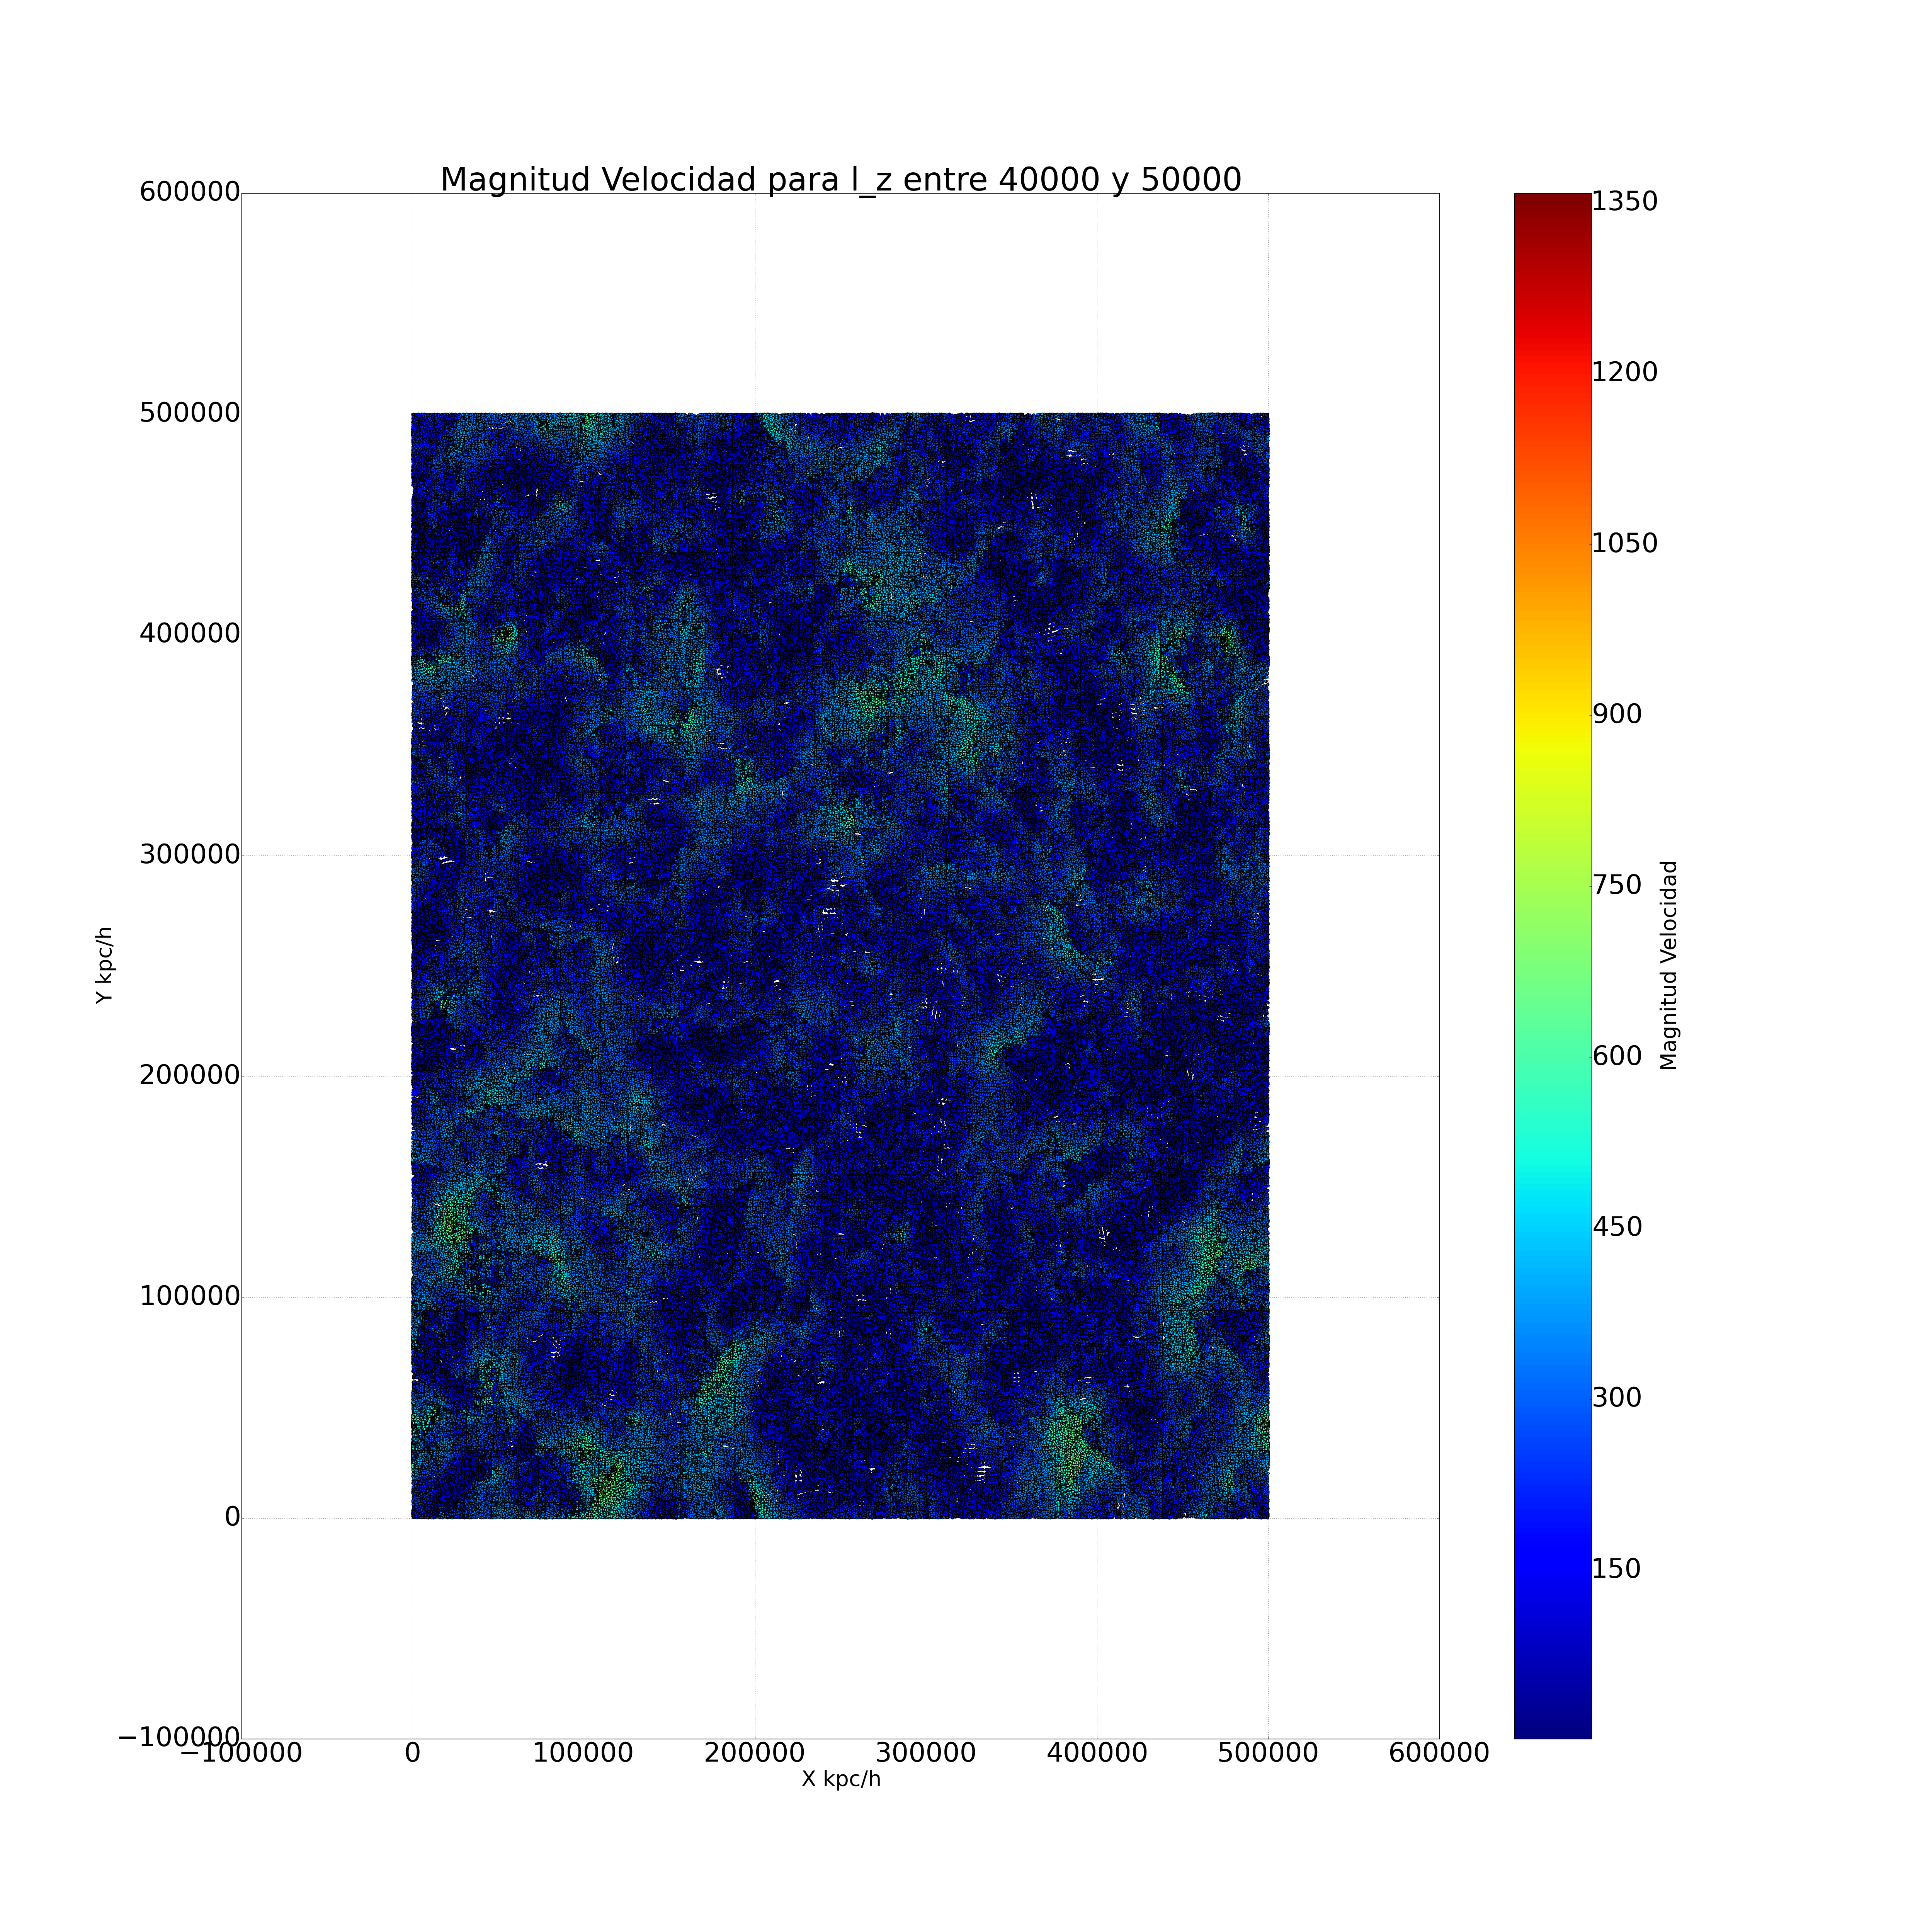
\includegraphics[width=0.9\textwidth]{graphs/scatter_magnitud_vel50000.png}
\end{minipage}%
\begin{minipage}{.45\textwidth}
  \centering
  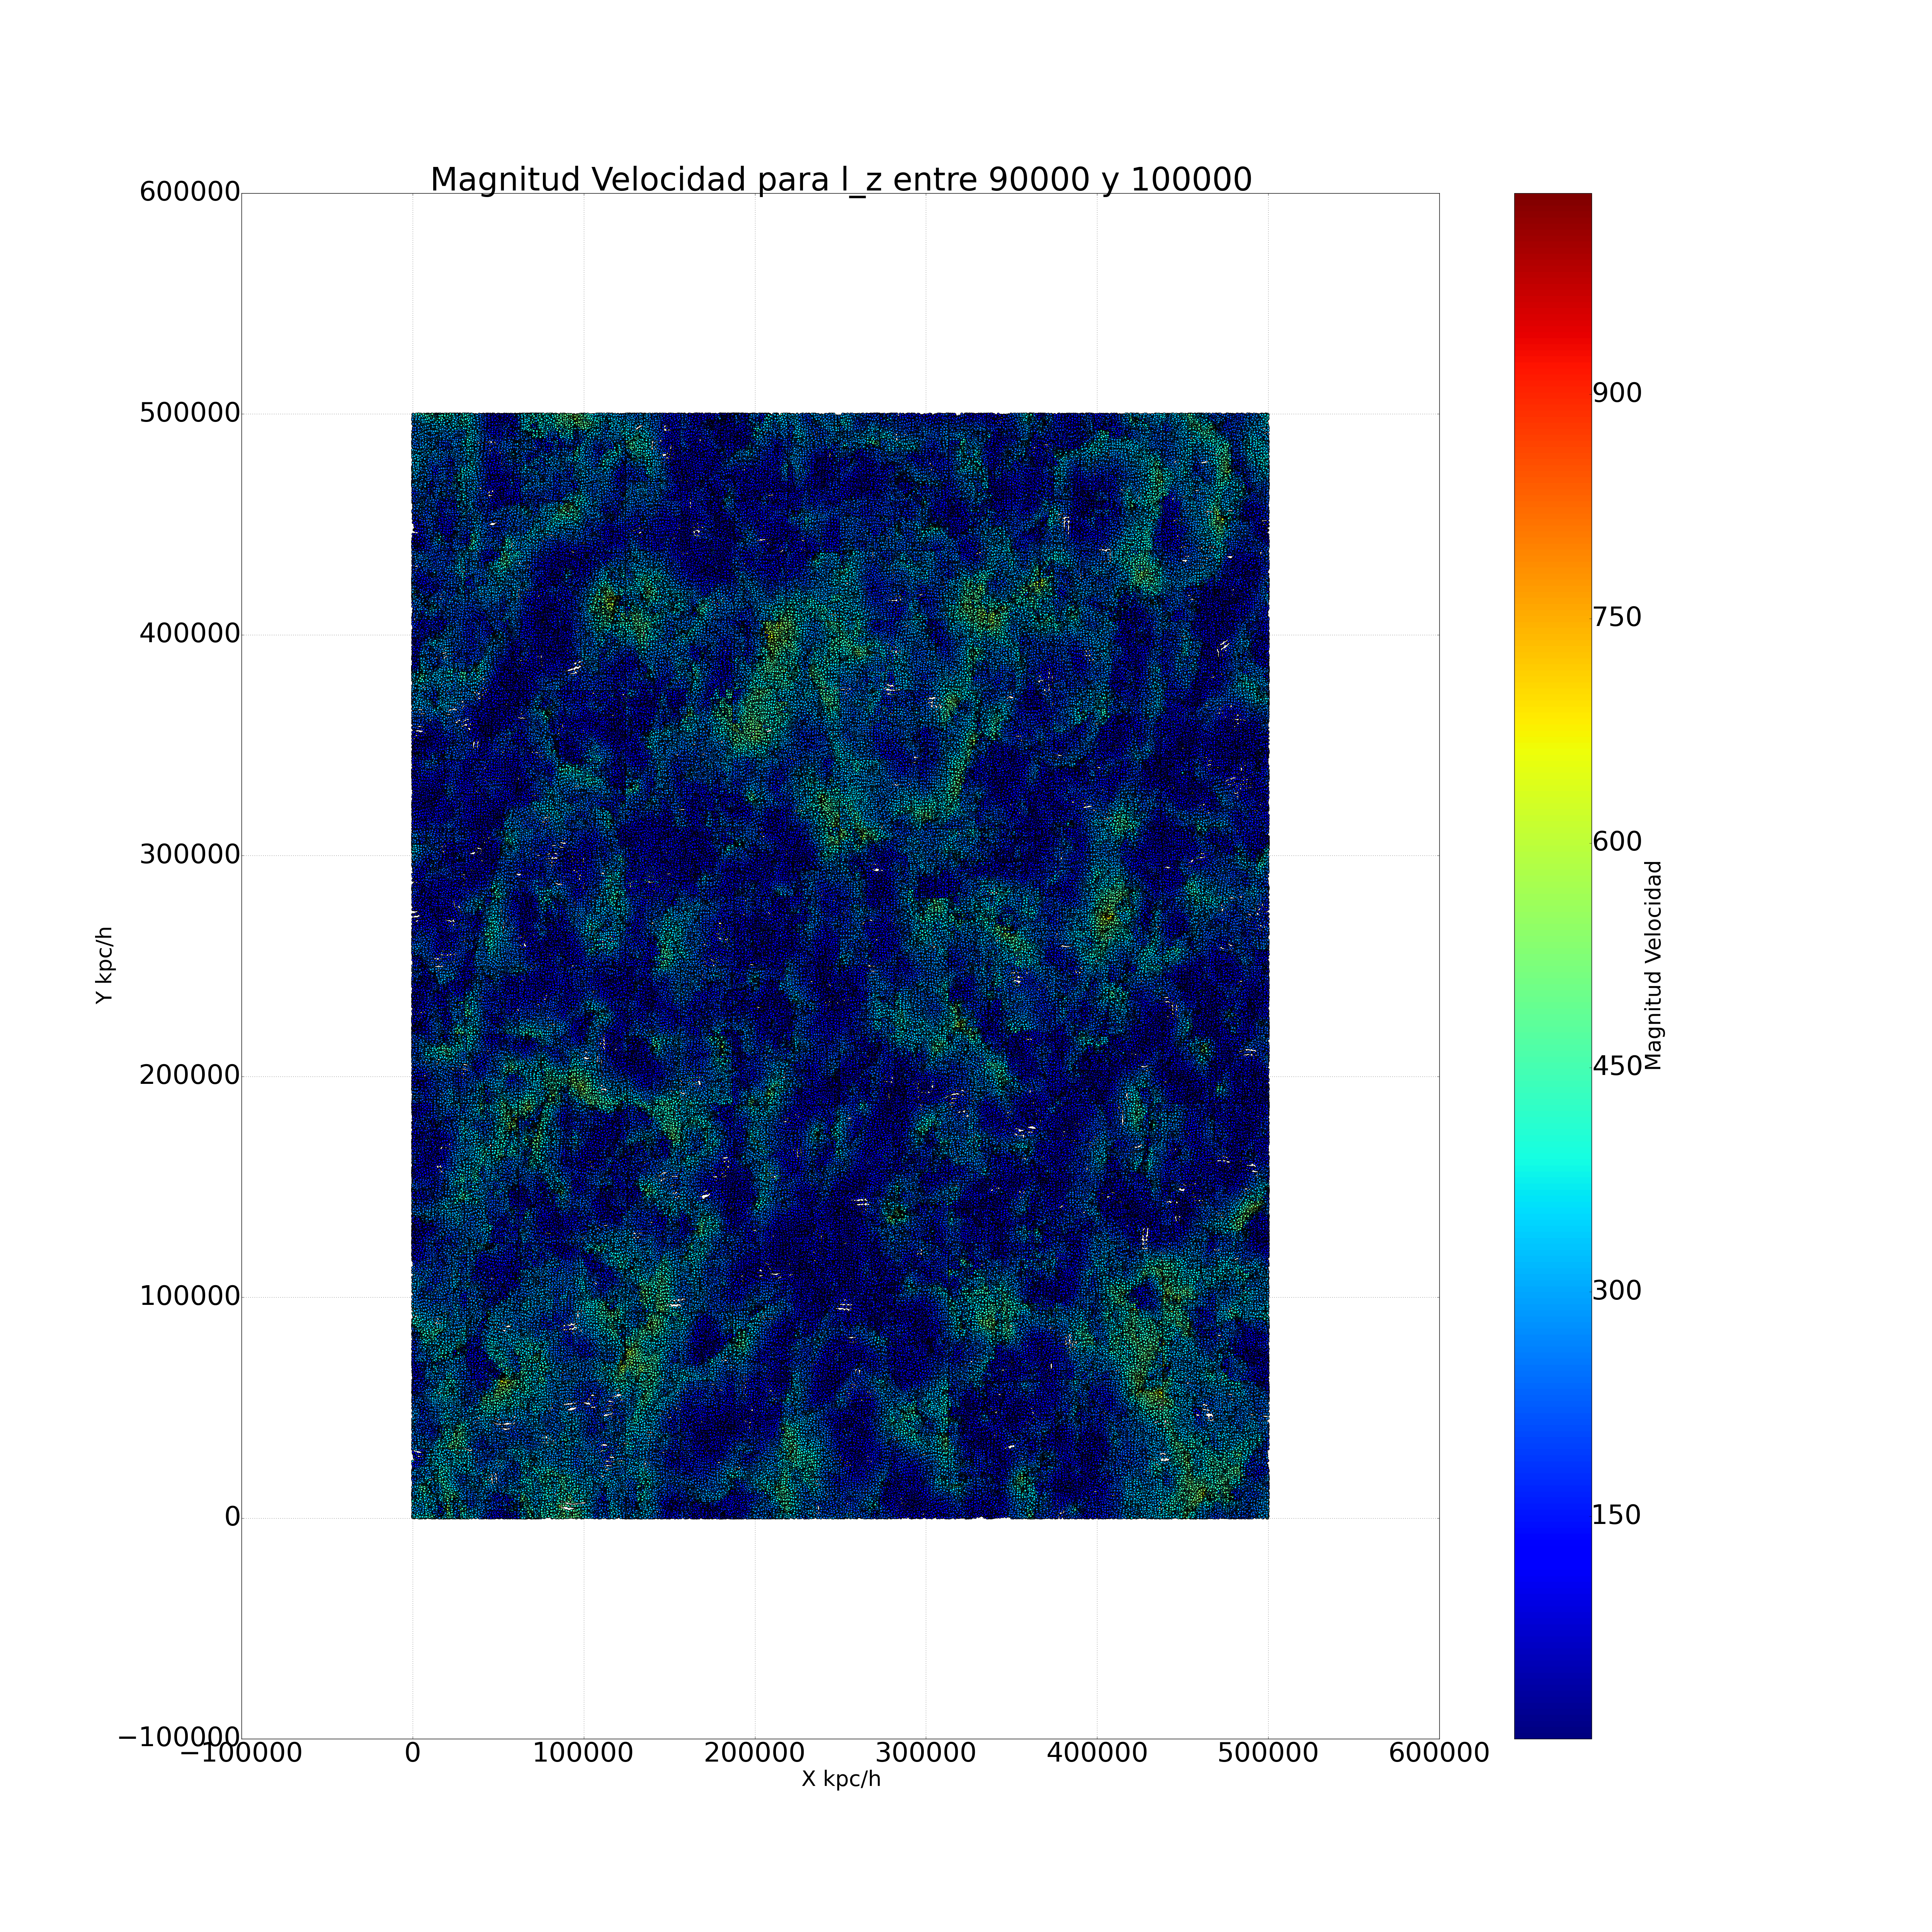
\includegraphics[width=0.9\textwidth]{graphs/scatter_magnitud_vel100000.png}
\end{minipage}
\begin{minipage}{.45\textwidth}
  \centering
  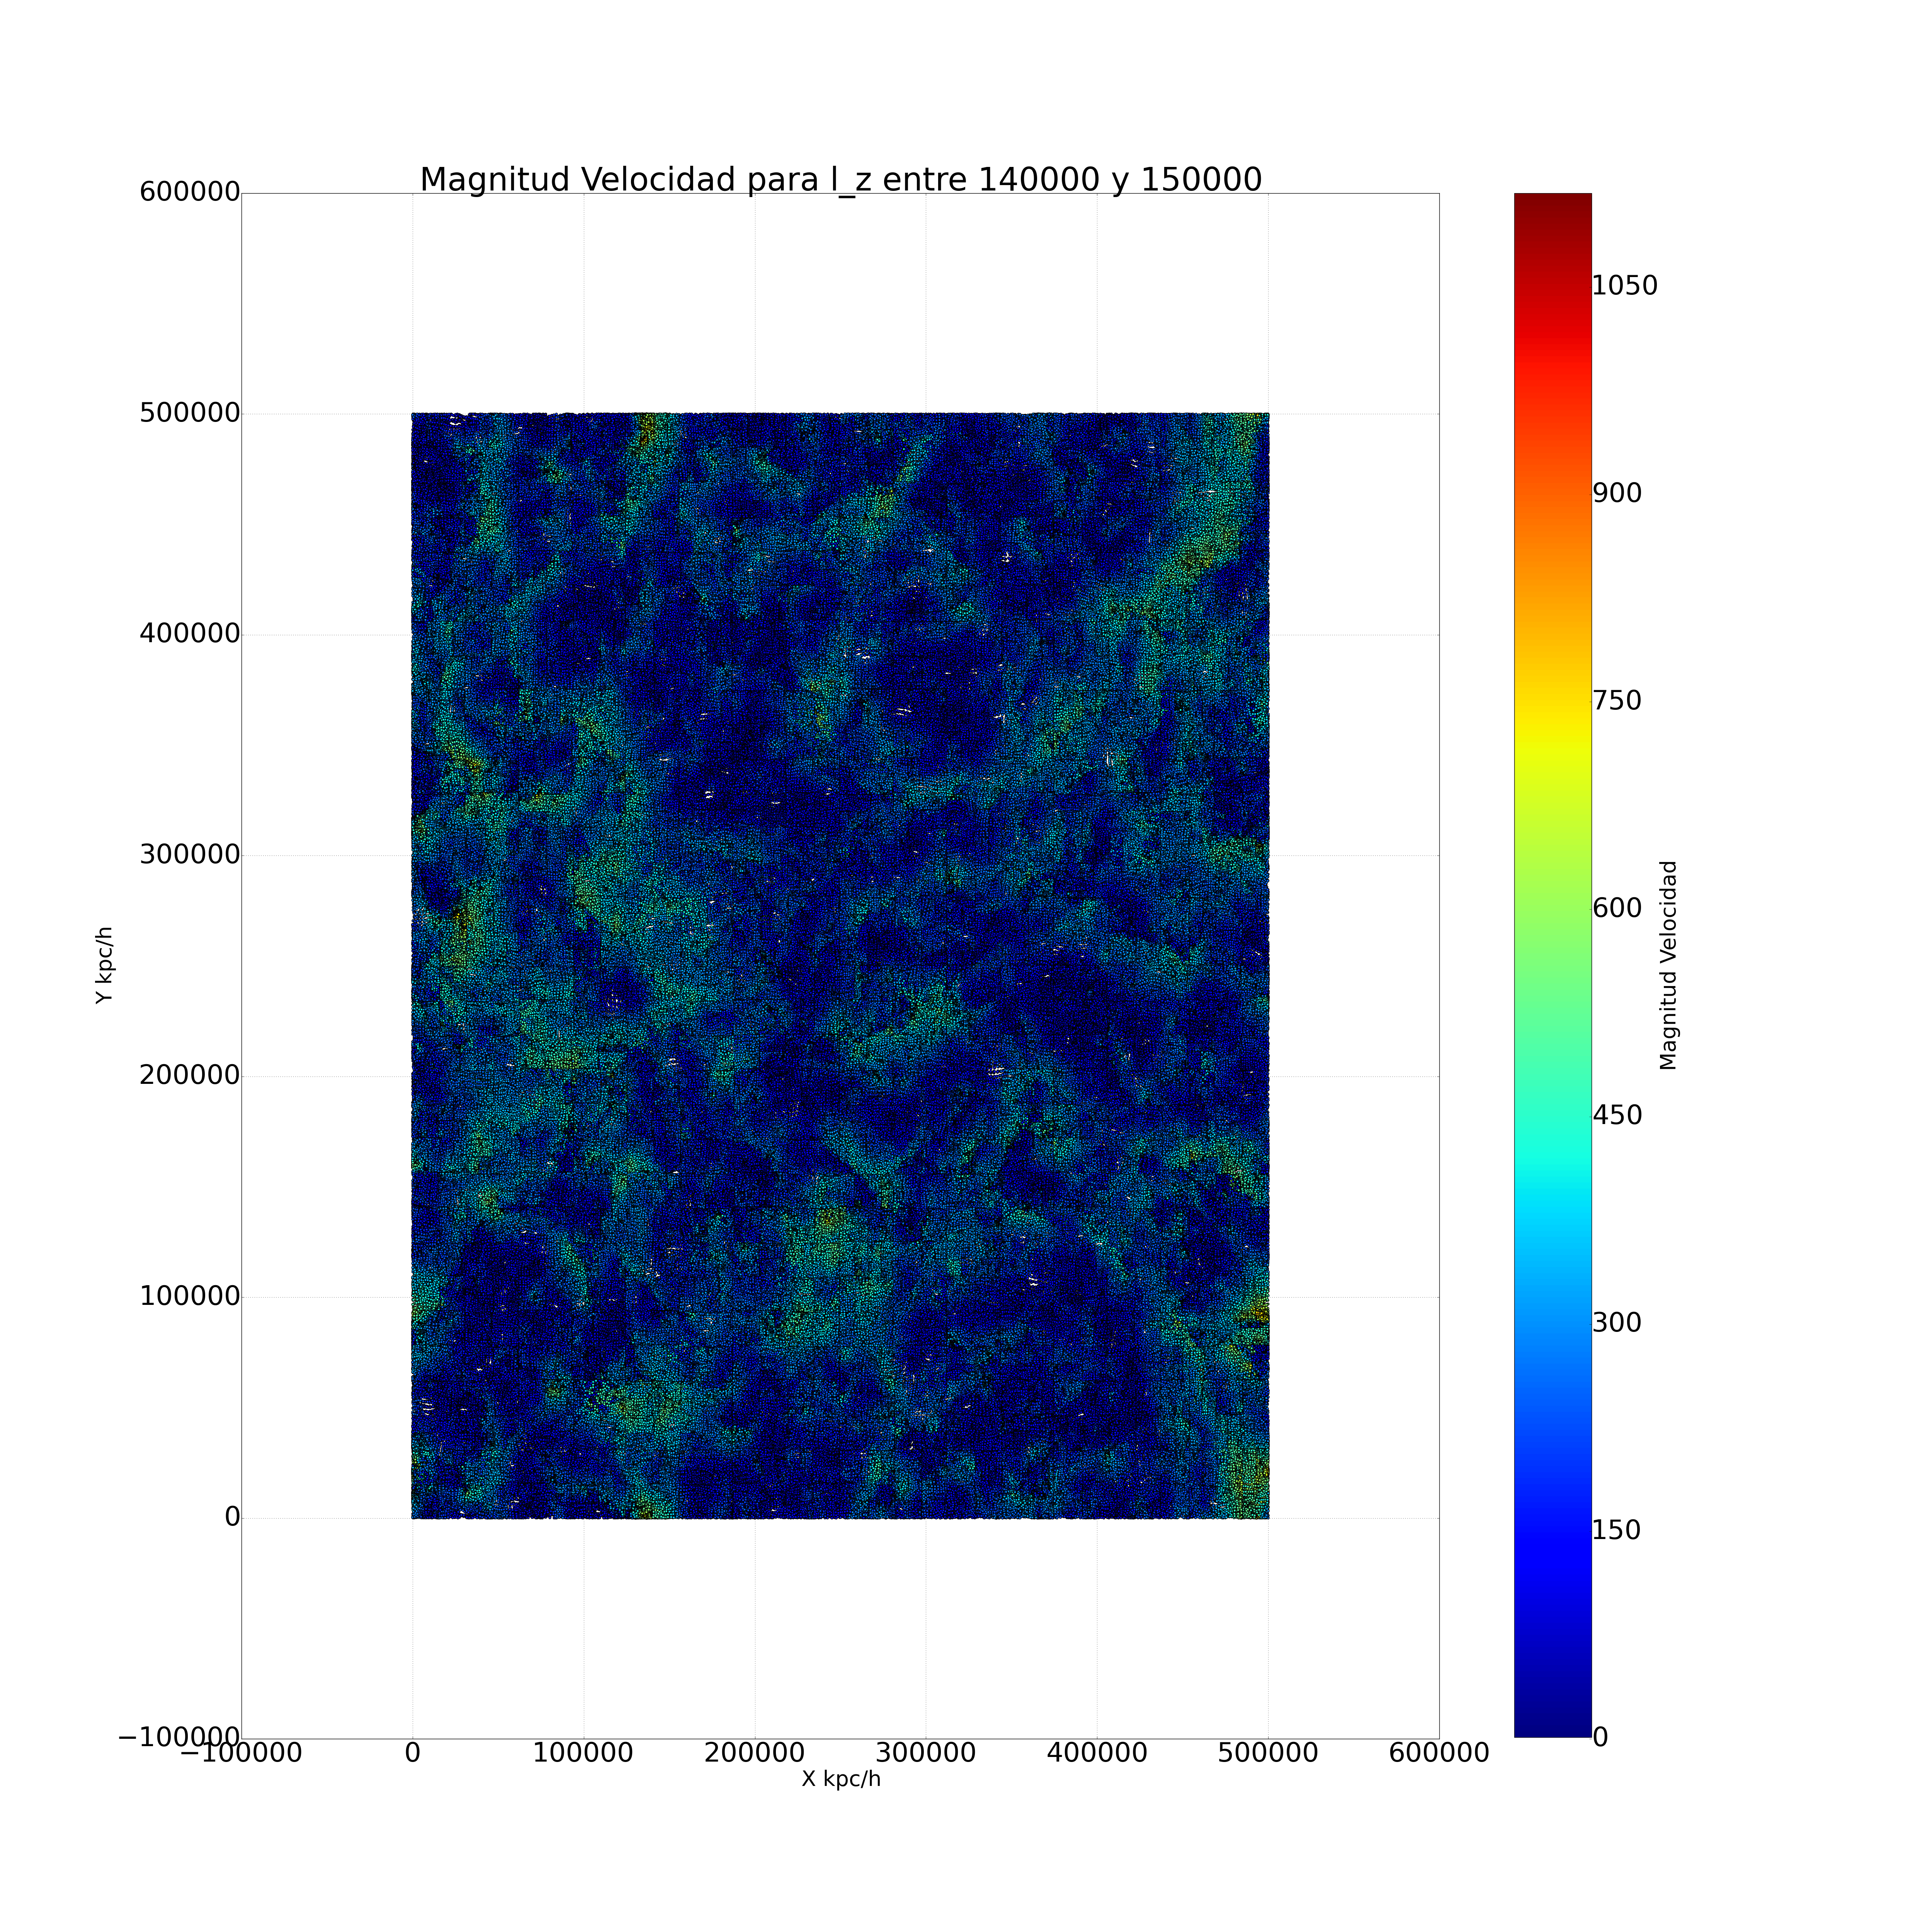
\includegraphics[width=0.9\textwidth]{graphs/scatter_magnitud_vel150000.png}
\end{minipage}
\begin{minipage}{.45\textwidth}
  \centering
  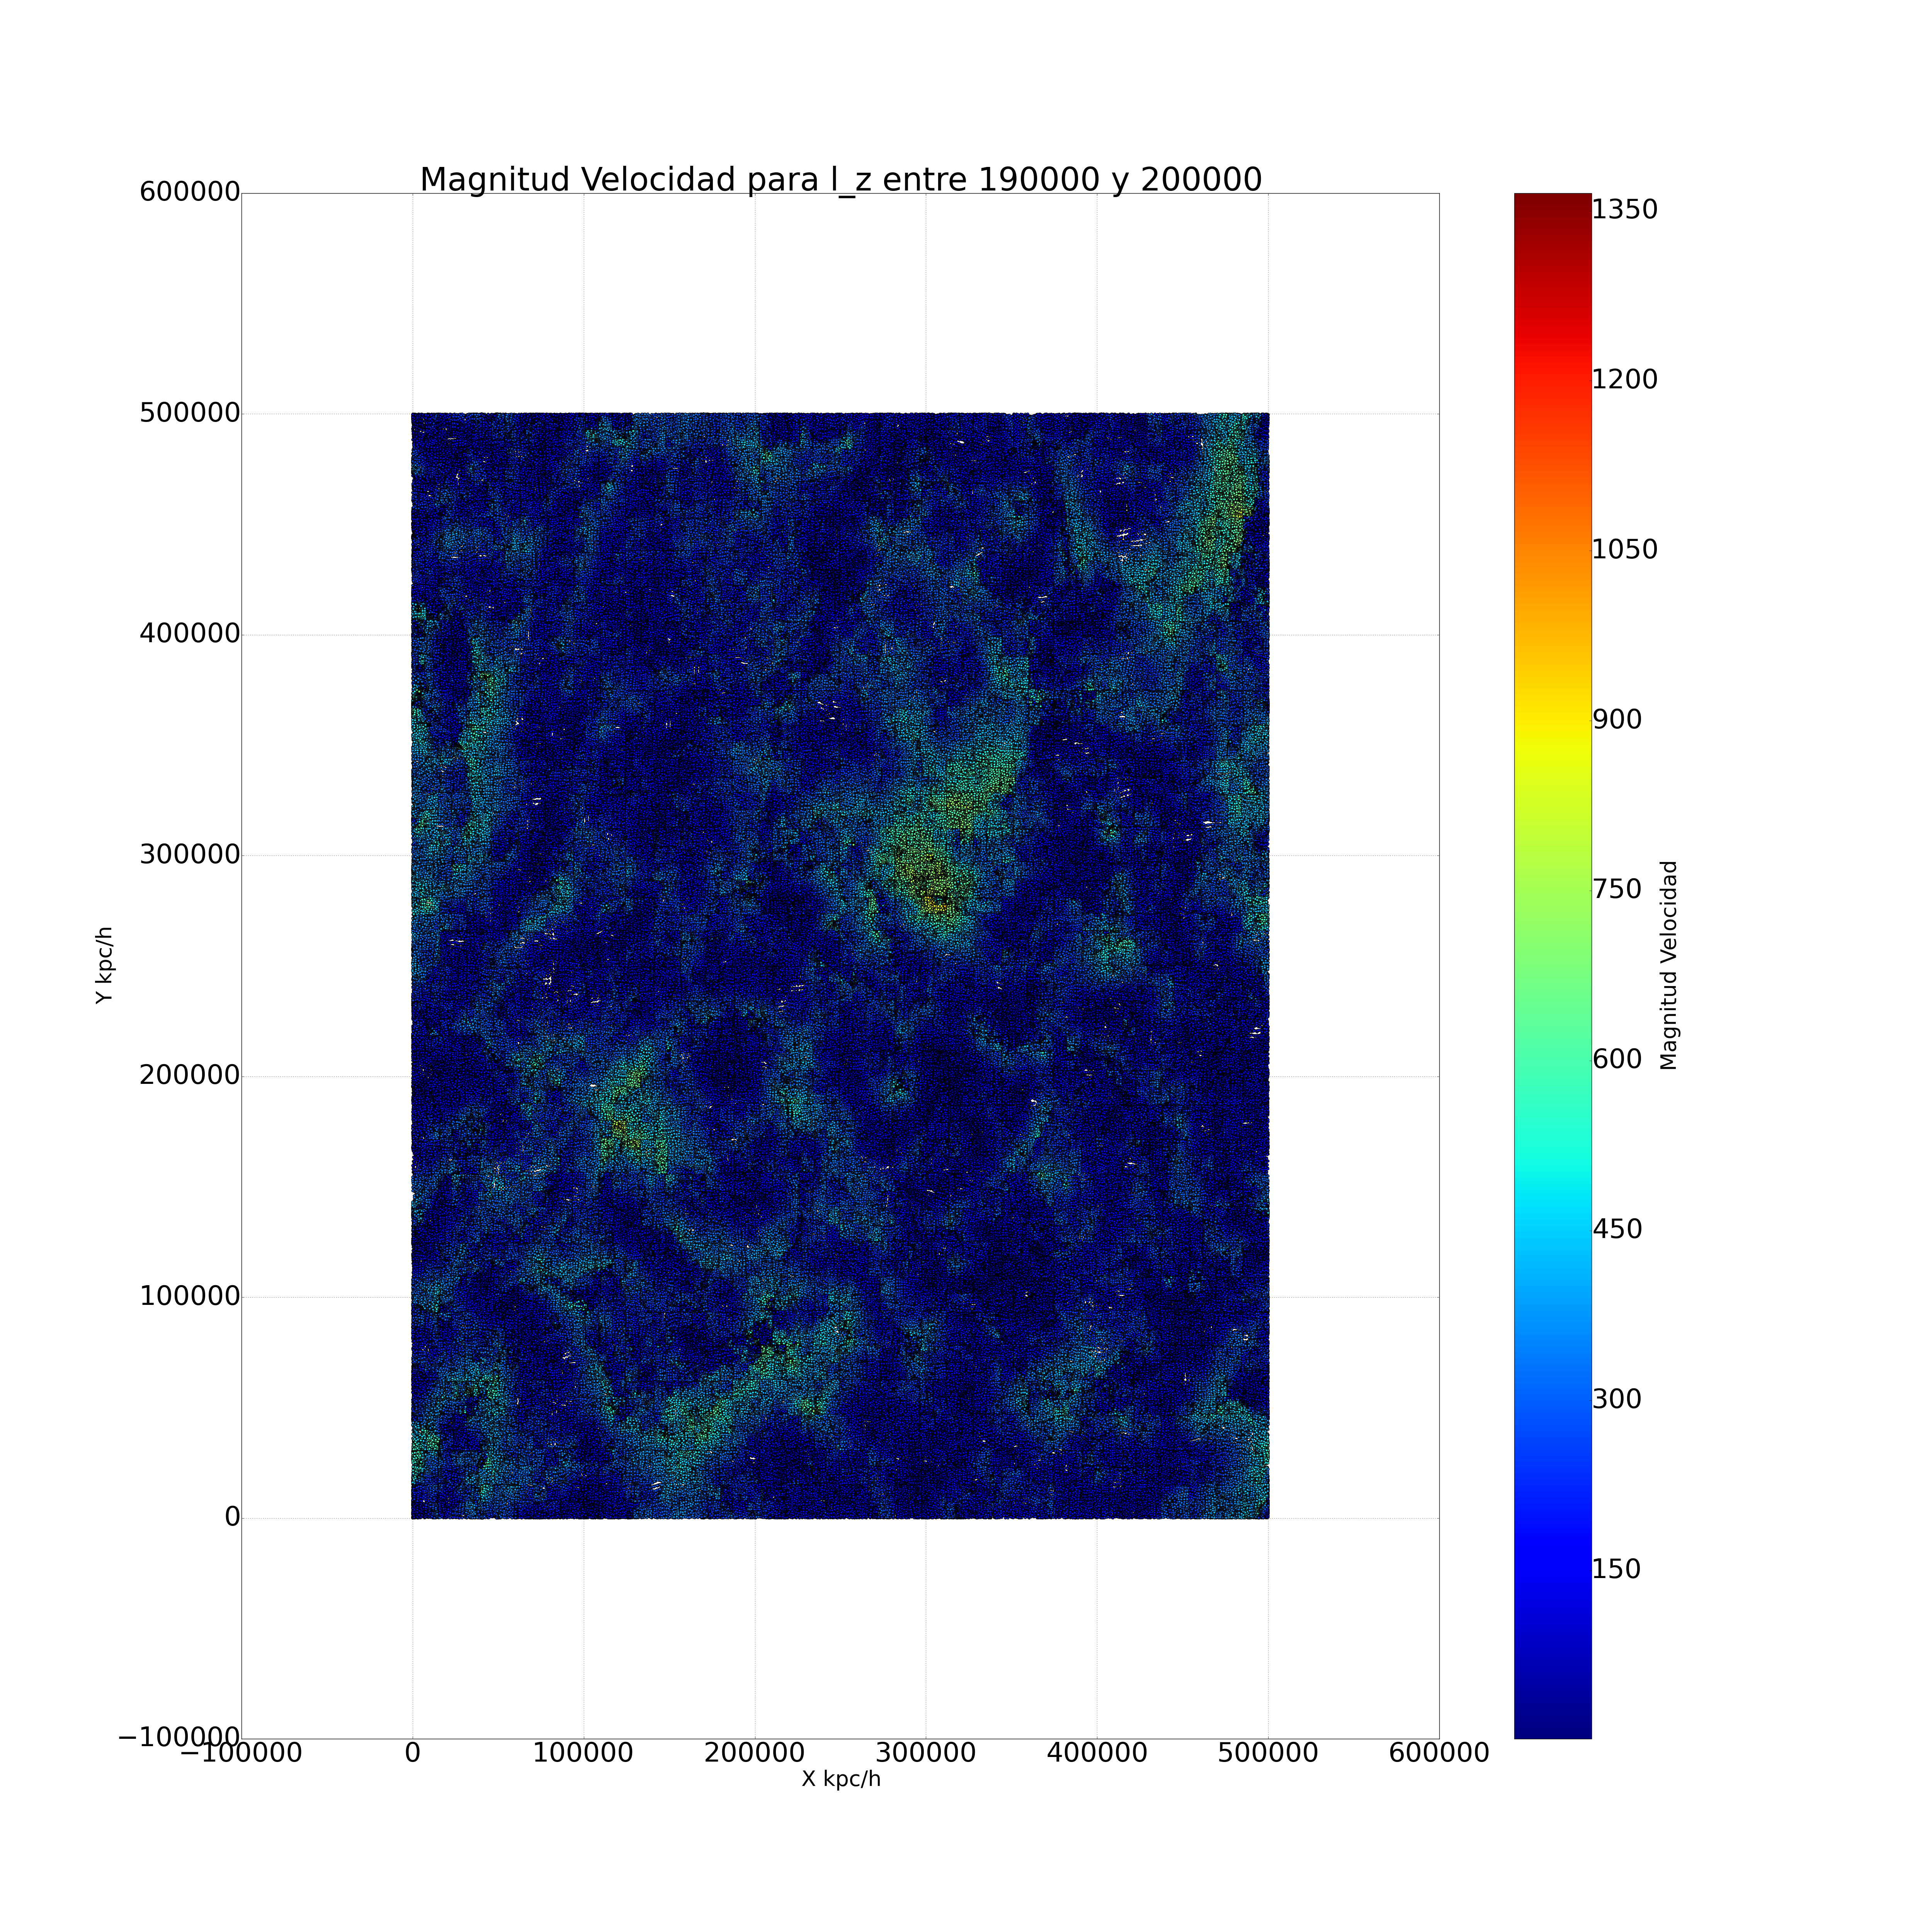
\includegraphics[width=0.9\textwidth]{graphs/scatter_magnitud_vel200000.png}
\end{minipage}
\caption{2D slices of the speed distribution}\label{fig:2D_slices}
\end{figure}
\FloatBarrier


We can observe in figure \ref{fig:2D_slices} intuitive signs of structures related to the speed distribution. 
We can observe filament structures\\

It is more clear if we observe from one side the particles with speed greater than a $th_{high}$ and the particles with speed lesser than a $th_{low}$.\\

\begin{figure}[ht]
\centering
\begin{minipage}{.45\textwidth}
  \centering
  \includegraphics[width=0.9\textwidth]{graphs/scatter_magnitud_vel_488_lz_100000.png}
\end{minipage}%
\begin{minipage}{.45\textwidth}
  \centering
  \includegraphics[width=0.9\textwidth]{graphs/scatter_magnitud_vel_488_lz_200000.png}
\end{minipage}
\begin{minipage}{.45\textwidth}
  \centering
  \includegraphics[width=0.9\textwidth]{graphs/scatter_magnitud_vel_59_lz_100000.png}
\end{minipage}
\begin{minipage}{.45\textwidth}
  \centering
  \includegraphics[width=0.9\textwidth]{graphs/scatter_magnitud_vel_59_lz_200000.png}
\end{minipage}
\caption{2D slices of the speed distribution. The upper slices with $|\vec{v}| > th_{high} = 488$ and the two lower slices with $|\vec{v}| < th_{low} = 59$ for the same cuts, $z = \{100, 200 \} Mpc/h$  }\label{fig:2D_slices_thresh}
\end{figure}
\FloatBarrier

As we can see in figure \ref{fig:2D_slices_thresh} the cuts with low and high thresholds are complementary. It is evident that structures are present. 

Finally we apply our region growing algorithm and we obtain the following results.\\

%Plot of the region identified.
\begin{figure}[ht]
\begin{center}
\includegraphics[width=0.8\textwidth]{graphs/regions_small.png} % Include the image placeholder.png
\caption{Region identified by the algorithm}
\label{fg:regions_speed_th_1}
\end{center}
\end{figure}
\FloatBarrier

And, changing the thresholds to: 
$th_{low} = \bar{v} + 2  \sigma_{v} = 488.48$ and $th_{high} = \bar{v}  +  8 \sigma_{v} =1195.0 $\\
We obtain:
%Plot of the region identified.
\begin{figure}[ht]
\begin{center}
\includegraphics[width=0.8\textwidth]{graphs/regions_big.png} % Include the image placeholder.png
\caption{Region identified by the algorithm with the second thresholds}
\label{fg:regions_speed_th_2}
\end{center}
\end{figure}
\FloatBarrier

We have different observations:\\
\begin{enumerate}
	\item The details of the regions in figures \ref{fg:regions_speed_th_1} and \ref{fg:regions_speed_th_2} seem accurate with what we would expect. It is more dense in the center and less dense in the borders.
	\item The regions obtained have a dimension of only a few Mpc/h (Laniakea's dimension is two orders of magnitude higher). This could mean that Laniakea is atypical. 
    \item There is first only one region identified. This indicates than all the high velocity particles are congregated in only one region (the detected region). If we set lower $th_{high}$ we can see we get more regions. 
    \item This is certainly a good naive approach to the problem. Nevertheless for more accurate results it needs to be drastically changed.
\end{enumerate}

The script in Appendix \ref{App:App_speed_code} was executed in a student's
laptop and later on the HPC cluster. For a significant number of particles, the laptop limited memory (8GB) crashes. Running in the HPC solves this issue.


\subsubsection{Code example for Region Growing Algorithm - Approach by the Speed} \label{App:App_speed_code}
\tiny
\lstinputlisting[language=Python, caption=Region Growing Algorithm Code - Speed]{code/region_detection_document.py}



\subsection{Simple implementation of the Region Growing Algorithm with the FA and VDH}

\subsubsection{Code example for Region Growing Algorithm - Approach by the FA and VDH}
\label{App:own_impl_code}
\tiny
\lstinputlisting[language=Python, caption=Region Growing Algorithm Code - FA \& VDH]{code/region_detection_FA_VDH_document.py}

\normalsize
\subsubsection{Region Growing Algorithm with the FA and VDH} \label{sec:results_own_impl}

\begin{par}
The results from the simple implementation are good. Nevertheless, our implementation using the FoF is much more efficient. We show this simple implementation and its results in a way to illustrate the concepts behind the Region Growing Algorithm.
\end{par}

\begin{par}
Using the data from our Small(Dense) simulation described in
 table \ref{tab:sims}, after the CIC (in a
  $256^3$ grid) and V-Web have been applied,
   we run the implementation described in section
    \ref{sec:own_impl_descr} for some of the
     values described in tables
      \ref{tab:seeds_FA_Trace} and
       \ref{tab:search_FA_Trace}. 
\end{par}

\begin{figure}[ht]
\begin{center}
\includegraphics[width=0.7\textwidth]{groups/firstimplementation/regions_3D_129.png} % Include the image placeholder.png
\caption{Regions detected for: Seeds (FA:0.6, VDH: 1.0) and Growth (FA:0.8, VDH: 0.0) }
\label{fg:first_3D_all}
\end{center}
\end{figure}
\FloatBarrier

\begin{figure}[ht]
\centering
\begin{minipage}{.5\textwidth}
  \centering
  \includegraphics[width=0.8\textwidth]{groups/firstimplementation/largest_vol_24_seeds_129.png} % Include the image placeholder.png
\end{minipage}%
\begin{minipage}{.5\textwidth}
  \centering
  \includegraphics[width=0.8\textwidth]{groups/firstimplementation/largest_vol_24_seeds_129_scale.png}
  \end{minipage}
\caption{Largest volume detected for: Seeds (FA:0.6, VDH: 1.0) and Growth (FA:0.8, VDH: 0.0). The region is on the left and can be seen at scale with the simulation on the right.}
\label{fg:first_3D_largest}
\end{figure}
\FloatBarrier


\end{document} 